\section{Le principe de la modulation}
\subsection{Présentation}
L'objectif de ce chapitre est de comprendre comment un signal peut-être transmis sur un canal.

\exemple{Un son, des données numériques, \dots{} sont des signaux.}
\exemple{Un câble coaxial, une ligne bifilaire, des ondes électromagnétiques, \dots{} sont des canaux}

La modulation permet de 
\begin{itemize}
  \item transporter plusieurs signaux sur un canal
  \item adapter la fréquence du signal pour qu'elle soit compatible avec le canal.
\end{itemize}

La modulation consiste à combiner 
\begin{itemize}
  \item le signal qu'on souhaite transmettre
  \item un signal sinusoïdal dont la fréquence est adaptée au canal appelé <<porteuse>>
\end{itemize}

\subsection{Les différents types de modulation}
\formule{Porteuse}[]
{$$s_p(t)=A_p\cos(2\pi f_pt+\phi_p)$$}
[
  \begin{itemize}
    \item $s_p(t)$ la porteuse
    \item $A_p$ l'amplitude de la porteuse
    \item $f_p$ la fréquence de la porteuse
    \item $\phi_p$ la phase de la porteuse
  \end{itemize}
]

Les trois types de modulation consistent à faire varier un de ces paramètres au cours du temps.

\subsubsection{La modulation d'amplitude}
La modulation d'amplitude consiste à faire varier l'amplitude de la porteuse : $A_p$ devient $A(t)$.

$$s_{AM}(t) = A(t)\cos(2\pi f_p t + \phi_p)$$

\begin{center}
  %% Creator: Matplotlib, PGF backend
%%
%% To include the figure in your LaTeX document, write
%%   \input{<filename>.pgf}
%%
%% Make sure the required packages are loaded in your preamble
%%   \usepackage{pgf}
%%
%% Also ensure that all the required font packages are loaded; for instance,
%% the lmodern package is sometimes necessary when using math font.
%%   \usepackage{lmodern}
%%
%% Figures using additional raster images can only be included by \input if
%% they are in the same directory as the main LaTeX file. For loading figures
%% from other directories you can use the `import` package
%%   \usepackage{import}
%%
%% and then include the figures with
%%   \import{<path to file>}{<filename>.pgf}
%%
%% Matplotlib used the following preamble
%%
\begingroup%
\makeatletter%
\begin{pgfpicture}%
\pgfpathrectangle{\pgfpointorigin}{\pgfqpoint{4.000000in}{2.000000in}}%
\pgfusepath{use as bounding box, clip}%
\begin{pgfscope}%
\pgfsetbuttcap%
\pgfsetmiterjoin%
\definecolor{currentfill}{rgb}{1.000000,1.000000,1.000000}%
\pgfsetfillcolor{currentfill}%
\pgfsetlinewidth{0.000000pt}%
\definecolor{currentstroke}{rgb}{1.000000,1.000000,1.000000}%
\pgfsetstrokecolor{currentstroke}%
\pgfsetdash{}{0pt}%
\pgfpathmoveto{\pgfqpoint{0.000000in}{0.000000in}}%
\pgfpathlineto{\pgfqpoint{4.000000in}{0.000000in}}%
\pgfpathlineto{\pgfqpoint{4.000000in}{2.000000in}}%
\pgfpathlineto{\pgfqpoint{0.000000in}{2.000000in}}%
\pgfpathlineto{\pgfqpoint{0.000000in}{0.000000in}}%
\pgfpathclose%
\pgfusepath{fill}%
\end{pgfscope}%
\begin{pgfscope}%
\pgfsetbuttcap%
\pgfsetmiterjoin%
\definecolor{currentfill}{rgb}{1.000000,1.000000,1.000000}%
\pgfsetfillcolor{currentfill}%
\pgfsetlinewidth{0.000000pt}%
\definecolor{currentstroke}{rgb}{0.000000,0.000000,0.000000}%
\pgfsetstrokecolor{currentstroke}%
\pgfsetstrokeopacity{0.000000}%
\pgfsetdash{}{0pt}%
\pgfpathmoveto{\pgfqpoint{0.500000in}{1.060000in}}%
\pgfpathlineto{\pgfqpoint{3.600000in}{1.060000in}}%
\pgfpathlineto{\pgfqpoint{3.600000in}{1.760000in}}%
\pgfpathlineto{\pgfqpoint{0.500000in}{1.760000in}}%
\pgfpathlineto{\pgfqpoint{0.500000in}{1.060000in}}%
\pgfpathclose%
\pgfusepath{fill}%
\end{pgfscope}%
\begin{pgfscope}%
\definecolor{textcolor}{rgb}{0.000000,0.000000,0.000000}%
\pgfsetstrokecolor{textcolor}%
\pgfsetfillcolor{textcolor}%
\pgftext[x=0.395833in,y=1.410000in,,bottom,rotate=90.000000]{\color{textcolor}\rmfamily\fontsize{10.000000}{12.000000}\selectfont signal modulant}%
\end{pgfscope}%
\begin{pgfscope}%
\pgfpathrectangle{\pgfqpoint{0.500000in}{1.060000in}}{\pgfqpoint{3.100000in}{0.700000in}}%
\pgfusepath{clip}%
\pgfsetrectcap%
\pgfsetroundjoin%
\pgfsetlinewidth{1.505625pt}%
\definecolor{currentstroke}{rgb}{0.121569,0.466667,0.705882}%
\pgfsetstrokecolor{currentstroke}%
\pgfsetdash{}{0pt}%
\pgfpathmoveto{\pgfqpoint{0.640909in}{1.728182in}}%
\pgfpathlineto{\pgfqpoint{1.343339in}{1.728182in}}%
\pgfpathlineto{\pgfqpoint{1.346160in}{1.091818in}}%
\pgfpathlineto{\pgfqpoint{2.048589in}{1.091818in}}%
\pgfpathlineto{\pgfqpoint{2.051411in}{1.728182in}}%
\pgfpathlineto{\pgfqpoint{2.753840in}{1.728182in}}%
\pgfpathlineto{\pgfqpoint{2.756661in}{1.091818in}}%
\pgfpathlineto{\pgfqpoint{3.456270in}{1.091818in}}%
\pgfpathlineto{\pgfqpoint{3.459091in}{1.728182in}}%
\pgfpathlineto{\pgfqpoint{3.459091in}{1.728182in}}%
\pgfusepath{stroke}%
\end{pgfscope}%
\begin{pgfscope}%
\pgfsetrectcap%
\pgfsetmiterjoin%
\pgfsetlinewidth{0.803000pt}%
\definecolor{currentstroke}{rgb}{0.000000,0.000000,0.000000}%
\pgfsetstrokecolor{currentstroke}%
\pgfsetdash{}{0pt}%
\pgfpathmoveto{\pgfqpoint{0.500000in}{1.060000in}}%
\pgfpathlineto{\pgfqpoint{0.500000in}{1.760000in}}%
\pgfusepath{stroke}%
\end{pgfscope}%
\begin{pgfscope}%
\pgfsetrectcap%
\pgfsetmiterjoin%
\pgfsetlinewidth{0.803000pt}%
\definecolor{currentstroke}{rgb}{0.000000,0.000000,0.000000}%
\pgfsetstrokecolor{currentstroke}%
\pgfsetdash{}{0pt}%
\pgfpathmoveto{\pgfqpoint{3.600000in}{1.060000in}}%
\pgfpathlineto{\pgfqpoint{3.600000in}{1.760000in}}%
\pgfusepath{stroke}%
\end{pgfscope}%
\begin{pgfscope}%
\pgfsetrectcap%
\pgfsetmiterjoin%
\pgfsetlinewidth{0.803000pt}%
\definecolor{currentstroke}{rgb}{0.000000,0.000000,0.000000}%
\pgfsetstrokecolor{currentstroke}%
\pgfsetdash{}{0pt}%
\pgfpathmoveto{\pgfqpoint{0.500000in}{1.060000in}}%
\pgfpathlineto{\pgfqpoint{3.600000in}{1.060000in}}%
\pgfusepath{stroke}%
\end{pgfscope}%
\begin{pgfscope}%
\pgfsetrectcap%
\pgfsetmiterjoin%
\pgfsetlinewidth{0.803000pt}%
\definecolor{currentstroke}{rgb}{0.000000,0.000000,0.000000}%
\pgfsetstrokecolor{currentstroke}%
\pgfsetdash{}{0pt}%
\pgfpathmoveto{\pgfqpoint{0.500000in}{1.760000in}}%
\pgfpathlineto{\pgfqpoint{3.600000in}{1.760000in}}%
\pgfusepath{stroke}%
\end{pgfscope}%
\begin{pgfscope}%
\definecolor{textcolor}{rgb}{0.000000,0.000000,0.000000}%
\pgfsetstrokecolor{textcolor}%
\pgfsetfillcolor{textcolor}%
\pgftext[x=2.050000in,y=1.843333in,,base]{\color{textcolor}\rmfamily\fontsize{12.000000}{14.400000}\selectfont Modulation en amplitude}%
\end{pgfscope}%
\begin{pgfscope}%
\pgfsetbuttcap%
\pgfsetmiterjoin%
\definecolor{currentfill}{rgb}{1.000000,1.000000,1.000000}%
\pgfsetfillcolor{currentfill}%
\pgfsetlinewidth{0.000000pt}%
\definecolor{currentstroke}{rgb}{0.000000,0.000000,0.000000}%
\pgfsetstrokecolor{currentstroke}%
\pgfsetstrokeopacity{0.000000}%
\pgfsetdash{}{0pt}%
\pgfpathmoveto{\pgfqpoint{0.500000in}{0.220000in}}%
\pgfpathlineto{\pgfqpoint{3.600000in}{0.220000in}}%
\pgfpathlineto{\pgfqpoint{3.600000in}{0.920000in}}%
\pgfpathlineto{\pgfqpoint{0.500000in}{0.920000in}}%
\pgfpathlineto{\pgfqpoint{0.500000in}{0.220000in}}%
\pgfpathclose%
\pgfusepath{fill}%
\end{pgfscope}%
\begin{pgfscope}%
\definecolor{textcolor}{rgb}{0.000000,0.000000,0.000000}%
\pgfsetstrokecolor{textcolor}%
\pgfsetfillcolor{textcolor}%
\pgftext[x=2.050000in,y=0.115833in,,top]{\color{textcolor}\rmfamily\fontsize{10.000000}{12.000000}\selectfont temps (s)}%
\end{pgfscope}%
\begin{pgfscope}%
\definecolor{textcolor}{rgb}{0.000000,0.000000,0.000000}%
\pgfsetstrokecolor{textcolor}%
\pgfsetfillcolor{textcolor}%
\pgftext[x=0.395833in,y=0.570000in,,bottom,rotate=90.000000]{\color{textcolor}\rmfamily\fontsize{10.000000}{12.000000}\selectfont signal modulé}%
\end{pgfscope}%
\begin{pgfscope}%
\pgfpathrectangle{\pgfqpoint{0.500000in}{0.220000in}}{\pgfqpoint{3.100000in}{0.700000in}}%
\pgfusepath{clip}%
\pgfsetrectcap%
\pgfsetroundjoin%
\pgfsetlinewidth{1.505625pt}%
\definecolor{currentstroke}{rgb}{0.121569,0.466667,0.705882}%
\pgfsetstrokecolor{currentstroke}%
\pgfsetdash{}{0pt}%
\pgfpathmoveto{\pgfqpoint{0.640909in}{0.888182in}}%
\pgfpathlineto{\pgfqpoint{0.643730in}{0.885668in}}%
\pgfpathlineto{\pgfqpoint{0.646551in}{0.878166in}}%
\pgfpathlineto{\pgfqpoint{0.652193in}{0.848748in}}%
\pgfpathlineto{\pgfqpoint{0.657835in}{0.801780in}}%
\pgfpathlineto{\pgfqpoint{0.666298in}{0.705149in}}%
\pgfpathlineto{\pgfqpoint{0.694508in}{0.337534in}}%
\pgfpathlineto{\pgfqpoint{0.700150in}{0.290770in}}%
\pgfpathlineto{\pgfqpoint{0.705792in}{0.261585in}}%
\pgfpathlineto{\pgfqpoint{0.708613in}{0.254207in}}%
\pgfpathlineto{\pgfqpoint{0.711434in}{0.251818in}}%
\pgfpathlineto{\pgfqpoint{0.714255in}{0.254458in}}%
\pgfpathlineto{\pgfqpoint{0.717076in}{0.262083in}}%
\pgfpathlineto{\pgfqpoint{0.722718in}{0.291735in}}%
\pgfpathlineto{\pgfqpoint{0.728360in}{0.338905in}}%
\pgfpathlineto{\pgfqpoint{0.736823in}{0.435756in}}%
\pgfpathlineto{\pgfqpoint{0.765033in}{0.803146in}}%
\pgfpathlineto{\pgfqpoint{0.770675in}{0.849707in}}%
\pgfpathlineto{\pgfqpoint{0.776317in}{0.878658in}}%
\pgfpathlineto{\pgfqpoint{0.779138in}{0.885913in}}%
\pgfpathlineto{\pgfqpoint{0.781959in}{0.888176in}}%
\pgfpathlineto{\pgfqpoint{0.784780in}{0.885411in}}%
\pgfpathlineto{\pgfqpoint{0.787601in}{0.877661in}}%
\pgfpathlineto{\pgfqpoint{0.793243in}{0.847777in}}%
\pgfpathlineto{\pgfqpoint{0.798885in}{0.800404in}}%
\pgfpathlineto{\pgfqpoint{0.807348in}{0.703334in}}%
\pgfpathlineto{\pgfqpoint{0.835558in}{0.336172in}}%
\pgfpathlineto{\pgfqpoint{0.841200in}{0.289816in}}%
\pgfpathlineto{\pgfqpoint{0.846842in}{0.261099in}}%
\pgfpathlineto{\pgfqpoint{0.849663in}{0.253968in}}%
\pgfpathlineto{\pgfqpoint{0.852484in}{0.251831in}}%
\pgfpathlineto{\pgfqpoint{0.855305in}{0.254721in}}%
\pgfpathlineto{\pgfqpoint{0.858126in}{0.262594in}}%
\pgfpathlineto{\pgfqpoint{0.863768in}{0.292711in}}%
\pgfpathlineto{\pgfqpoint{0.869410in}{0.340285in}}%
\pgfpathlineto{\pgfqpoint{0.877873in}{0.437573in}}%
\pgfpathlineto{\pgfqpoint{0.906083in}{0.804504in}}%
\pgfpathlineto{\pgfqpoint{0.911725in}{0.850655in}}%
\pgfpathlineto{\pgfqpoint{0.917367in}{0.879138in}}%
\pgfpathlineto{\pgfqpoint{0.920188in}{0.886145in}}%
\pgfpathlineto{\pgfqpoint{0.923009in}{0.888157in}}%
\pgfpathlineto{\pgfqpoint{0.925830in}{0.885141in}}%
\pgfpathlineto{\pgfqpoint{0.928651in}{0.877145in}}%
\pgfpathlineto{\pgfqpoint{0.934293in}{0.846796in}}%
\pgfpathlineto{\pgfqpoint{0.939935in}{0.799020in}}%
\pgfpathlineto{\pgfqpoint{0.948398in}{0.701515in}}%
\pgfpathlineto{\pgfqpoint{0.976608in}{0.334820in}}%
\pgfpathlineto{\pgfqpoint{0.982250in}{0.288873in}}%
\pgfpathlineto{\pgfqpoint{0.987892in}{0.260626in}}%
\pgfpathlineto{\pgfqpoint{0.990713in}{0.253742in}}%
\pgfpathlineto{\pgfqpoint{0.993534in}{0.251856in}}%
\pgfpathlineto{\pgfqpoint{0.996355in}{0.254997in}}%
\pgfpathlineto{\pgfqpoint{0.999176in}{0.263116in}}%
\pgfpathlineto{\pgfqpoint{1.004818in}{0.293698in}}%
\pgfpathlineto{\pgfqpoint{1.010460in}{0.341675in}}%
\pgfpathlineto{\pgfqpoint{1.018923in}{0.439395in}}%
\pgfpathlineto{\pgfqpoint{1.047133in}{0.805851in}}%
\pgfpathlineto{\pgfqpoint{1.052776in}{0.851593in}}%
\pgfpathlineto{\pgfqpoint{1.058418in}{0.879605in}}%
\pgfpathlineto{\pgfqpoint{1.061239in}{0.886365in}}%
\pgfpathlineto{\pgfqpoint{1.064060in}{0.888125in}}%
\pgfpathlineto{\pgfqpoint{1.066881in}{0.884858in}}%
\pgfpathlineto{\pgfqpoint{1.069702in}{0.876616in}}%
\pgfpathlineto{\pgfqpoint{1.075344in}{0.845803in}}%
\pgfpathlineto{\pgfqpoint{1.080986in}{0.797626in}}%
\pgfpathlineto{\pgfqpoint{1.089449in}{0.699690in}}%
\pgfpathlineto{\pgfqpoint{1.117659in}{0.333477in}}%
\pgfpathlineto{\pgfqpoint{1.123301in}{0.287941in}}%
\pgfpathlineto{\pgfqpoint{1.128943in}{0.260164in}}%
\pgfpathlineto{\pgfqpoint{1.131764in}{0.253528in}}%
\pgfpathlineto{\pgfqpoint{1.134585in}{0.251894in}}%
\pgfpathlineto{\pgfqpoint{1.137406in}{0.255286in}}%
\pgfpathlineto{\pgfqpoint{1.140227in}{0.263651in}}%
\pgfpathlineto{\pgfqpoint{1.145869in}{0.294695in}}%
\pgfpathlineto{\pgfqpoint{1.151511in}{0.343073in}}%
\pgfpathlineto{\pgfqpoint{1.159974in}{0.441223in}}%
\pgfpathlineto{\pgfqpoint{1.188184in}{0.807190in}}%
\pgfpathlineto{\pgfqpoint{1.193826in}{0.852519in}}%
\pgfpathlineto{\pgfqpoint{1.199468in}{0.880061in}}%
\pgfpathlineto{\pgfqpoint{1.202289in}{0.886572in}}%
\pgfpathlineto{\pgfqpoint{1.205110in}{0.888081in}}%
\pgfpathlineto{\pgfqpoint{1.207931in}{0.884564in}}%
\pgfpathlineto{\pgfqpoint{1.210752in}{0.876076in}}%
\pgfpathlineto{\pgfqpoint{1.216394in}{0.844800in}}%
\pgfpathlineto{\pgfqpoint{1.222036in}{0.796223in}}%
\pgfpathlineto{\pgfqpoint{1.230499in}{0.697860in}}%
\pgfpathlineto{\pgfqpoint{1.258709in}{0.332143in}}%
\pgfpathlineto{\pgfqpoint{1.264351in}{0.287021in}}%
\pgfpathlineto{\pgfqpoint{1.269993in}{0.259715in}}%
\pgfpathlineto{\pgfqpoint{1.272814in}{0.253327in}}%
\pgfpathlineto{\pgfqpoint{1.275635in}{0.251944in}}%
\pgfpathlineto{\pgfqpoint{1.278456in}{0.255587in}}%
\pgfpathlineto{\pgfqpoint{1.281277in}{0.264198in}}%
\pgfpathlineto{\pgfqpoint{1.286919in}{0.295704in}}%
\pgfpathlineto{\pgfqpoint{1.292561in}{0.344480in}}%
\pgfpathlineto{\pgfqpoint{1.301024in}{0.443055in}}%
\pgfpathlineto{\pgfqpoint{1.329234in}{0.808519in}}%
\pgfpathlineto{\pgfqpoint{1.334876in}{0.853434in}}%
\pgfpathlineto{\pgfqpoint{1.340518in}{0.880504in}}%
\pgfpathlineto{\pgfqpoint{1.343339in}{0.886767in}}%
\pgfpathlineto{\pgfqpoint{1.346160in}{0.741244in}}%
\pgfpathlineto{\pgfqpoint{1.348981in}{0.739215in}}%
\pgfpathlineto{\pgfqpoint{1.351802in}{0.734512in}}%
\pgfpathlineto{\pgfqpoint{1.357444in}{0.717423in}}%
\pgfpathlineto{\pgfqpoint{1.363086in}{0.691052in}}%
\pgfpathlineto{\pgfqpoint{1.371549in}{0.637859in}}%
\pgfpathlineto{\pgfqpoint{1.399759in}{0.441209in}}%
\pgfpathlineto{\pgfqpoint{1.405401in}{0.417137in}}%
\pgfpathlineto{\pgfqpoint{1.411043in}{0.402688in}}%
\pgfpathlineto{\pgfqpoint{1.413864in}{0.399382in}}%
\pgfpathlineto{\pgfqpoint{1.416685in}{0.398773in}}%
\pgfpathlineto{\pgfqpoint{1.419506in}{0.400869in}}%
\pgfpathlineto{\pgfqpoint{1.422327in}{0.405638in}}%
\pgfpathlineto{\pgfqpoint{1.427969in}{0.422851in}}%
\pgfpathlineto{\pgfqpoint{1.433611in}{0.449328in}}%
\pgfpathlineto{\pgfqpoint{1.442074in}{0.502634in}}%
\pgfpathlineto{\pgfqpoint{1.470284in}{0.699144in}}%
\pgfpathlineto{\pgfqpoint{1.475926in}{0.723104in}}%
\pgfpathlineto{\pgfqpoint{1.481568in}{0.737426in}}%
\pgfpathlineto{\pgfqpoint{1.484389in}{0.740665in}}%
\pgfpathlineto{\pgfqpoint{1.487210in}{0.741206in}}%
\pgfpathlineto{\pgfqpoint{1.490031in}{0.739043in}}%
\pgfpathlineto{\pgfqpoint{1.492852in}{0.734208in}}%
\pgfpathlineto{\pgfqpoint{1.498494in}{0.716871in}}%
\pgfpathlineto{\pgfqpoint{1.504136in}{0.690287in}}%
\pgfpathlineto{\pgfqpoint{1.512599in}{0.636868in}}%
\pgfpathlineto{\pgfqpoint{1.540809in}{0.440501in}}%
\pgfpathlineto{\pgfqpoint{1.546451in}{0.416653in}}%
\pgfpathlineto{\pgfqpoint{1.552093in}{0.402459in}}%
\pgfpathlineto{\pgfqpoint{1.554914in}{0.399287in}}%
\pgfpathlineto{\pgfqpoint{1.557735in}{0.398813in}}%
\pgfpathlineto{\pgfqpoint{1.560556in}{0.401044in}}%
\pgfpathlineto{\pgfqpoint{1.563377in}{0.405945in}}%
\pgfpathlineto{\pgfqpoint{1.569019in}{0.423406in}}%
\pgfpathlineto{\pgfqpoint{1.574661in}{0.450096in}}%
\pgfpathlineto{\pgfqpoint{1.583124in}{0.503626in}}%
\pgfpathlineto{\pgfqpoint{1.611334in}{0.699849in}}%
\pgfpathlineto{\pgfqpoint{1.616976in}{0.723585in}}%
\pgfpathlineto{\pgfqpoint{1.622618in}{0.737651in}}%
\pgfpathlineto{\pgfqpoint{1.625439in}{0.740756in}}%
\pgfpathlineto{\pgfqpoint{1.628260in}{0.741162in}}%
\pgfpathlineto{\pgfqpoint{1.631081in}{0.738864in}}%
\pgfpathlineto{\pgfqpoint{1.633902in}{0.733897in}}%
\pgfpathlineto{\pgfqpoint{1.639544in}{0.716313in}}%
\pgfpathlineto{\pgfqpoint{1.645186in}{0.689517in}}%
\pgfpathlineto{\pgfqpoint{1.653649in}{0.635875in}}%
\pgfpathlineto{\pgfqpoint{1.681859in}{0.439798in}}%
\pgfpathlineto{\pgfqpoint{1.687501in}{0.416175in}}%
\pgfpathlineto{\pgfqpoint{1.693143in}{0.402237in}}%
\pgfpathlineto{\pgfqpoint{1.695964in}{0.399199in}}%
\pgfpathlineto{\pgfqpoint{1.698785in}{0.398861in}}%
\pgfpathlineto{\pgfqpoint{1.701606in}{0.401226in}}%
\pgfpathlineto{\pgfqpoint{1.704427in}{0.406259in}}%
\pgfpathlineto{\pgfqpoint{1.710069in}{0.423966in}}%
\pgfpathlineto{\pgfqpoint{1.715711in}{0.450868in}}%
\pgfpathlineto{\pgfqpoint{1.724174in}{0.504621in}}%
\pgfpathlineto{\pgfqpoint{1.752384in}{0.700550in}}%
\pgfpathlineto{\pgfqpoint{1.758026in}{0.724060in}}%
\pgfpathlineto{\pgfqpoint{1.763668in}{0.737870in}}%
\pgfpathlineto{\pgfqpoint{1.766489in}{0.740841in}}%
\pgfpathlineto{\pgfqpoint{1.769310in}{0.741111in}}%
\pgfpathlineto{\pgfqpoint{1.772131in}{0.738678in}}%
\pgfpathlineto{\pgfqpoint{1.774952in}{0.733580in}}%
\pgfpathlineto{\pgfqpoint{1.780594in}{0.715750in}}%
\pgfpathlineto{\pgfqpoint{1.786236in}{0.688743in}}%
\pgfpathlineto{\pgfqpoint{1.794699in}{0.634879in}}%
\pgfpathlineto{\pgfqpoint{1.820088in}{0.454003in}}%
\pgfpathlineto{\pgfqpoint{1.825730in}{0.426267in}}%
\pgfpathlineto{\pgfqpoint{1.831372in}{0.407579in}}%
\pgfpathlineto{\pgfqpoint{1.834193in}{0.402022in}}%
\pgfpathlineto{\pgfqpoint{1.837014in}{0.399118in}}%
\pgfpathlineto{\pgfqpoint{1.839835in}{0.398915in}}%
\pgfpathlineto{\pgfqpoint{1.842656in}{0.401415in}}%
\pgfpathlineto{\pgfqpoint{1.845477in}{0.406580in}}%
\pgfpathlineto{\pgfqpoint{1.851119in}{0.424533in}}%
\pgfpathlineto{\pgfqpoint{1.856761in}{0.451645in}}%
\pgfpathlineto{\pgfqpoint{1.865224in}{0.505618in}}%
\pgfpathlineto{\pgfqpoint{1.890613in}{0.686391in}}%
\pgfpathlineto{\pgfqpoint{1.896255in}{0.714024in}}%
\pgfpathlineto{\pgfqpoint{1.901897in}{0.732590in}}%
\pgfpathlineto{\pgfqpoint{1.904718in}{0.738082in}}%
\pgfpathlineto{\pgfqpoint{1.907539in}{0.740918in}}%
\pgfpathlineto{\pgfqpoint{1.910360in}{0.741054in}}%
\pgfpathlineto{\pgfqpoint{1.913181in}{0.738486in}}%
\pgfpathlineto{\pgfqpoint{1.916002in}{0.733256in}}%
\pgfpathlineto{\pgfqpoint{1.921644in}{0.715180in}}%
\pgfpathlineto{\pgfqpoint{1.927286in}{0.687964in}}%
\pgfpathlineto{\pgfqpoint{1.935749in}{0.633880in}}%
\pgfpathlineto{\pgfqpoint{1.961138in}{0.453212in}}%
\pgfpathlineto{\pgfqpoint{1.966780in}{0.425683in}}%
\pgfpathlineto{\pgfqpoint{1.972422in}{0.407240in}}%
\pgfpathlineto{\pgfqpoint{1.975243in}{0.401813in}}%
\pgfpathlineto{\pgfqpoint{1.978064in}{0.399044in}}%
\pgfpathlineto{\pgfqpoint{1.980885in}{0.398976in}}%
\pgfpathlineto{\pgfqpoint{1.983706in}{0.401611in}}%
\pgfpathlineto{\pgfqpoint{1.986527in}{0.406906in}}%
\pgfpathlineto{\pgfqpoint{1.992169in}{0.425105in}}%
\pgfpathlineto{\pgfqpoint{1.997811in}{0.452426in}}%
\pgfpathlineto{\pgfqpoint{2.006274in}{0.506618in}}%
\pgfpathlineto{\pgfqpoint{2.031663in}{0.687180in}}%
\pgfpathlineto{\pgfqpoint{2.037305in}{0.714605in}}%
\pgfpathlineto{\pgfqpoint{2.042947in}{0.732926in}}%
\pgfpathlineto{\pgfqpoint{2.045768in}{0.738288in}}%
\pgfpathlineto{\pgfqpoint{2.048589in}{0.740990in}}%
\pgfpathlineto{\pgfqpoint{2.051411in}{0.887553in}}%
\pgfpathlineto{\pgfqpoint{2.054232in}{0.882535in}}%
\pgfpathlineto{\pgfqpoint{2.057053in}{0.872578in}}%
\pgfpathlineto{\pgfqpoint{2.062695in}{0.838553in}}%
\pgfpathlineto{\pgfqpoint{2.068337in}{0.787620in}}%
\pgfpathlineto{\pgfqpoint{2.076800in}{0.686776in}}%
\pgfpathlineto{\pgfqpoint{2.102189in}{0.351649in}}%
\pgfpathlineto{\pgfqpoint{2.107831in}{0.300910in}}%
\pgfpathlineto{\pgfqpoint{2.113473in}{0.267113in}}%
\pgfpathlineto{\pgfqpoint{2.116294in}{0.257278in}}%
\pgfpathlineto{\pgfqpoint{2.119115in}{0.252384in}}%
\pgfpathlineto{\pgfqpoint{2.121936in}{0.252510in}}%
\pgfpathlineto{\pgfqpoint{2.124757in}{0.257653in}}%
\pgfpathlineto{\pgfqpoint{2.127578in}{0.267732in}}%
\pgfpathlineto{\pgfqpoint{2.133220in}{0.301983in}}%
\pgfpathlineto{\pgfqpoint{2.138862in}{0.353109in}}%
\pgfpathlineto{\pgfqpoint{2.147325in}{0.454153in}}%
\pgfpathlineto{\pgfqpoint{2.172714in}{0.789076in}}%
\pgfpathlineto{\pgfqpoint{2.178356in}{0.839621in}}%
\pgfpathlineto{\pgfqpoint{2.183998in}{0.873191in}}%
\pgfpathlineto{\pgfqpoint{2.186819in}{0.882904in}}%
\pgfpathlineto{\pgfqpoint{2.189640in}{0.887672in}}%
\pgfpathlineto{\pgfqpoint{2.192461in}{0.887421in}}%
\pgfpathlineto{\pgfqpoint{2.195282in}{0.882153in}}%
\pgfpathlineto{\pgfqpoint{2.198103in}{0.871953in}}%
\pgfpathlineto{\pgfqpoint{2.203745in}{0.837475in}}%
\pgfpathlineto{\pgfqpoint{2.209387in}{0.786156in}}%
\pgfpathlineto{\pgfqpoint{2.217850in}{0.684913in}}%
\pgfpathlineto{\pgfqpoint{2.243239in}{0.350198in}}%
\pgfpathlineto{\pgfqpoint{2.248881in}{0.299847in}}%
\pgfpathlineto{\pgfqpoint{2.254523in}{0.266505in}}%
\pgfpathlineto{\pgfqpoint{2.257344in}{0.256915in}}%
\pgfpathlineto{\pgfqpoint{2.260165in}{0.252271in}}%
\pgfpathlineto{\pgfqpoint{2.262986in}{0.252649in}}%
\pgfpathlineto{\pgfqpoint{2.265807in}{0.258041in}}%
\pgfpathlineto{\pgfqpoint{2.268628in}{0.268362in}}%
\pgfpathlineto{\pgfqpoint{2.274270in}{0.303067in}}%
\pgfpathlineto{\pgfqpoint{2.279912in}{0.354578in}}%
\pgfpathlineto{\pgfqpoint{2.288375in}{0.456019in}}%
\pgfpathlineto{\pgfqpoint{2.313764in}{0.790523in}}%
\pgfpathlineto{\pgfqpoint{2.319406in}{0.840678in}}%
\pgfpathlineto{\pgfqpoint{2.325048in}{0.873792in}}%
\pgfpathlineto{\pgfqpoint{2.327869in}{0.883261in}}%
\pgfpathlineto{\pgfqpoint{2.330690in}{0.887779in}}%
\pgfpathlineto{\pgfqpoint{2.333511in}{0.887276in}}%
\pgfpathlineto{\pgfqpoint{2.336332in}{0.881759in}}%
\pgfpathlineto{\pgfqpoint{2.339153in}{0.871316in}}%
\pgfpathlineto{\pgfqpoint{2.344795in}{0.836385in}}%
\pgfpathlineto{\pgfqpoint{2.350437in}{0.784683in}}%
\pgfpathlineto{\pgfqpoint{2.358900in}{0.683044in}}%
\pgfpathlineto{\pgfqpoint{2.384289in}{0.348755in}}%
\pgfpathlineto{\pgfqpoint{2.389931in}{0.298795in}}%
\pgfpathlineto{\pgfqpoint{2.395573in}{0.265910in}}%
\pgfpathlineto{\pgfqpoint{2.398394in}{0.256564in}}%
\pgfpathlineto{\pgfqpoint{2.401215in}{0.252171in}}%
\pgfpathlineto{\pgfqpoint{2.404036in}{0.252799in}}%
\pgfpathlineto{\pgfqpoint{2.406857in}{0.258441in}}%
\pgfpathlineto{\pgfqpoint{2.409678in}{0.269005in}}%
\pgfpathlineto{\pgfqpoint{2.415320in}{0.304162in}}%
\pgfpathlineto{\pgfqpoint{2.420962in}{0.356055in}}%
\pgfpathlineto{\pgfqpoint{2.429425in}{0.457890in}}%
\pgfpathlineto{\pgfqpoint{2.454814in}{0.791961in}}%
\pgfpathlineto{\pgfqpoint{2.460456in}{0.841725in}}%
\pgfpathlineto{\pgfqpoint{2.466098in}{0.874381in}}%
\pgfpathlineto{\pgfqpoint{2.468919in}{0.883605in}}%
\pgfpathlineto{\pgfqpoint{2.471740in}{0.887873in}}%
\pgfpathlineto{\pgfqpoint{2.474561in}{0.887119in}}%
\pgfpathlineto{\pgfqpoint{2.477382in}{0.881353in}}%
\pgfpathlineto{\pgfqpoint{2.480203in}{0.870667in}}%
\pgfpathlineto{\pgfqpoint{2.485845in}{0.835286in}}%
\pgfpathlineto{\pgfqpoint{2.491487in}{0.783202in}}%
\pgfpathlineto{\pgfqpoint{2.499950in}{0.681171in}}%
\pgfpathlineto{\pgfqpoint{2.525339in}{0.347321in}}%
\pgfpathlineto{\pgfqpoint{2.530981in}{0.297754in}}%
\pgfpathlineto{\pgfqpoint{2.536623in}{0.265327in}}%
\pgfpathlineto{\pgfqpoint{2.539444in}{0.256226in}}%
\pgfpathlineto{\pgfqpoint{2.542265in}{0.252082in}}%
\pgfpathlineto{\pgfqpoint{2.545086in}{0.252963in}}%
\pgfpathlineto{\pgfqpoint{2.547907in}{0.258853in}}%
\pgfpathlineto{\pgfqpoint{2.550728in}{0.269660in}}%
\pgfpathlineto{\pgfqpoint{2.556370in}{0.305266in}}%
\pgfpathlineto{\pgfqpoint{2.562012in}{0.357540in}}%
\pgfpathlineto{\pgfqpoint{2.570475in}{0.459765in}}%
\pgfpathlineto{\pgfqpoint{2.595864in}{0.793391in}}%
\pgfpathlineto{\pgfqpoint{2.601506in}{0.842761in}}%
\pgfpathlineto{\pgfqpoint{2.607148in}{0.874958in}}%
\pgfpathlineto{\pgfqpoint{2.609969in}{0.883937in}}%
\pgfpathlineto{\pgfqpoint{2.612790in}{0.887955in}}%
\pgfpathlineto{\pgfqpoint{2.615611in}{0.886949in}}%
\pgfpathlineto{\pgfqpoint{2.618432in}{0.880934in}}%
\pgfpathlineto{\pgfqpoint{2.621253in}{0.870006in}}%
\pgfpathlineto{\pgfqpoint{2.626895in}{0.834176in}}%
\pgfpathlineto{\pgfqpoint{2.632537in}{0.781712in}}%
\pgfpathlineto{\pgfqpoint{2.641000in}{0.679294in}}%
\pgfpathlineto{\pgfqpoint{2.666389in}{0.345896in}}%
\pgfpathlineto{\pgfqpoint{2.672031in}{0.296724in}}%
\pgfpathlineto{\pgfqpoint{2.677673in}{0.264757in}}%
\pgfpathlineto{\pgfqpoint{2.680494in}{0.255900in}}%
\pgfpathlineto{\pgfqpoint{2.683315in}{0.252007in}}%
\pgfpathlineto{\pgfqpoint{2.686136in}{0.253139in}}%
\pgfpathlineto{\pgfqpoint{2.688957in}{0.259278in}}%
\pgfpathlineto{\pgfqpoint{2.691778in}{0.270327in}}%
\pgfpathlineto{\pgfqpoint{2.697420in}{0.306382in}}%
\pgfpathlineto{\pgfqpoint{2.703062in}{0.359034in}}%
\pgfpathlineto{\pgfqpoint{2.711525in}{0.461645in}}%
\pgfpathlineto{\pgfqpoint{2.736914in}{0.794811in}}%
\pgfpathlineto{\pgfqpoint{2.742556in}{0.843786in}}%
\pgfpathlineto{\pgfqpoint{2.748198in}{0.875523in}}%
\pgfpathlineto{\pgfqpoint{2.751019in}{0.884257in}}%
\pgfpathlineto{\pgfqpoint{2.753840in}{0.888024in}}%
\pgfpathlineto{\pgfqpoint{2.756661in}{0.740566in}}%
\pgfpathlineto{\pgfqpoint{2.759482in}{0.737194in}}%
\pgfpathlineto{\pgfqpoint{2.765124in}{0.722618in}}%
\pgfpathlineto{\pgfqpoint{2.770766in}{0.698433in}}%
\pgfpathlineto{\pgfqpoint{2.779229in}{0.647613in}}%
\pgfpathlineto{\pgfqpoint{2.810260in}{0.434362in}}%
\pgfpathlineto{\pgfqpoint{2.815902in}{0.412576in}}%
\pgfpathlineto{\pgfqpoint{2.821544in}{0.400700in}}%
\pgfpathlineto{\pgfqpoint{2.824365in}{0.398739in}}%
\pgfpathlineto{\pgfqpoint{2.827186in}{0.399484in}}%
\pgfpathlineto{\pgfqpoint{2.830007in}{0.402923in}}%
\pgfpathlineto{\pgfqpoint{2.835649in}{0.417626in}}%
\pgfpathlineto{\pgfqpoint{2.841291in}{0.441923in}}%
\pgfpathlineto{\pgfqpoint{2.849754in}{0.492866in}}%
\pgfpathlineto{\pgfqpoint{2.880785in}{0.705965in}}%
\pgfpathlineto{\pgfqpoint{2.886427in}{0.727635in}}%
\pgfpathlineto{\pgfqpoint{2.892069in}{0.739380in}}%
\pgfpathlineto{\pgfqpoint{2.894890in}{0.741274in}}%
\pgfpathlineto{\pgfqpoint{2.897711in}{0.740462in}}%
\pgfpathlineto{\pgfqpoint{2.900532in}{0.736955in}}%
\pgfpathlineto{\pgfqpoint{2.906174in}{0.722125in}}%
\pgfpathlineto{\pgfqpoint{2.911816in}{0.697717in}}%
\pgfpathlineto{\pgfqpoint{2.920279in}{0.646651in}}%
\pgfpathlineto{\pgfqpoint{2.951310in}{0.433707in}}%
\pgfpathlineto{\pgfqpoint{2.956952in}{0.412153in}}%
\pgfpathlineto{\pgfqpoint{2.962594in}{0.400538in}}%
\pgfpathlineto{\pgfqpoint{2.965415in}{0.398712in}}%
\pgfpathlineto{\pgfqpoint{2.968236in}{0.399592in}}%
\pgfpathlineto{\pgfqpoint{2.971057in}{0.403165in}}%
\pgfpathlineto{\pgfqpoint{2.976699in}{0.418122in}}%
\pgfpathlineto{\pgfqpoint{2.982341in}{0.442641in}}%
\pgfpathlineto{\pgfqpoint{2.990804in}{0.493830in}}%
\pgfpathlineto{\pgfqpoint{3.021835in}{0.706618in}}%
\pgfpathlineto{\pgfqpoint{3.027477in}{0.728054in}}%
\pgfpathlineto{\pgfqpoint{3.033119in}{0.739539in}}%
\pgfpathlineto{\pgfqpoint{3.035940in}{0.741298in}}%
\pgfpathlineto{\pgfqpoint{3.038761in}{0.740350in}}%
\pgfpathlineto{\pgfqpoint{3.041582in}{0.736710in}}%
\pgfpathlineto{\pgfqpoint{3.047224in}{0.721626in}}%
\pgfpathlineto{\pgfqpoint{3.052867in}{0.696997in}}%
\pgfpathlineto{\pgfqpoint{3.061330in}{0.645686in}}%
\pgfpathlineto{\pgfqpoint{3.092361in}{0.433056in}}%
\pgfpathlineto{\pgfqpoint{3.098003in}{0.411738in}}%
\pgfpathlineto{\pgfqpoint{3.103645in}{0.400383in}}%
\pgfpathlineto{\pgfqpoint{3.106466in}{0.398691in}}%
\pgfpathlineto{\pgfqpoint{3.109287in}{0.399707in}}%
\pgfpathlineto{\pgfqpoint{3.112108in}{0.403413in}}%
\pgfpathlineto{\pgfqpoint{3.117750in}{0.418624in}}%
\pgfpathlineto{\pgfqpoint{3.123392in}{0.443364in}}%
\pgfpathlineto{\pgfqpoint{3.131855in}{0.494797in}}%
\pgfpathlineto{\pgfqpoint{3.162886in}{0.707265in}}%
\pgfpathlineto{\pgfqpoint{3.168528in}{0.728466in}}%
\pgfpathlineto{\pgfqpoint{3.174170in}{0.739691in}}%
\pgfpathlineto{\pgfqpoint{3.176991in}{0.741315in}}%
\pgfpathlineto{\pgfqpoint{3.179812in}{0.740232in}}%
\pgfpathlineto{\pgfqpoint{3.182633in}{0.736458in}}%
\pgfpathlineto{\pgfqpoint{3.188275in}{0.721122in}}%
\pgfpathlineto{\pgfqpoint{3.193917in}{0.696271in}}%
\pgfpathlineto{\pgfqpoint{3.202380in}{0.644717in}}%
\pgfpathlineto{\pgfqpoint{3.233411in}{0.432411in}}%
\pgfpathlineto{\pgfqpoint{3.239053in}{0.411328in}}%
\pgfpathlineto{\pgfqpoint{3.244695in}{0.400234in}}%
\pgfpathlineto{\pgfqpoint{3.247516in}{0.398678in}}%
\pgfpathlineto{\pgfqpoint{3.250337in}{0.399829in}}%
\pgfpathlineto{\pgfqpoint{3.253158in}{0.403668in}}%
\pgfpathlineto{\pgfqpoint{3.258800in}{0.419131in}}%
\pgfpathlineto{\pgfqpoint{3.264442in}{0.444092in}}%
\pgfpathlineto{\pgfqpoint{3.272905in}{0.495766in}}%
\pgfpathlineto{\pgfqpoint{3.303936in}{0.707907in}}%
\pgfpathlineto{\pgfqpoint{3.309578in}{0.728873in}}%
\pgfpathlineto{\pgfqpoint{3.315220in}{0.739836in}}%
\pgfpathlineto{\pgfqpoint{3.318041in}{0.741325in}}%
\pgfpathlineto{\pgfqpoint{3.320862in}{0.740106in}}%
\pgfpathlineto{\pgfqpoint{3.323683in}{0.736200in}}%
\pgfpathlineto{\pgfqpoint{3.329325in}{0.720611in}}%
\pgfpathlineto{\pgfqpoint{3.334967in}{0.695540in}}%
\pgfpathlineto{\pgfqpoint{3.343430in}{0.643746in}}%
\pgfpathlineto{\pgfqpoint{3.374461in}{0.431772in}}%
\pgfpathlineto{\pgfqpoint{3.380103in}{0.410925in}}%
\pgfpathlineto{\pgfqpoint{3.385745in}{0.400092in}}%
\pgfpathlineto{\pgfqpoint{3.388566in}{0.398671in}}%
\pgfpathlineto{\pgfqpoint{3.391387in}{0.399957in}}%
\pgfpathlineto{\pgfqpoint{3.394208in}{0.403930in}}%
\pgfpathlineto{\pgfqpoint{3.399850in}{0.419645in}}%
\pgfpathlineto{\pgfqpoint{3.405492in}{0.444826in}}%
\pgfpathlineto{\pgfqpoint{3.413955in}{0.496739in}}%
\pgfpathlineto{\pgfqpoint{3.442165in}{0.694804in}}%
\pgfpathlineto{\pgfqpoint{3.447807in}{0.720094in}}%
\pgfpathlineto{\pgfqpoint{3.453449in}{0.735935in}}%
\pgfpathlineto{\pgfqpoint{3.456270in}{0.739975in}}%
\pgfpathlineto{\pgfqpoint{3.459091in}{0.888182in}}%
\pgfpathlineto{\pgfqpoint{3.459091in}{0.888182in}}%
\pgfusepath{stroke}%
\end{pgfscope}%
\begin{pgfscope}%
\pgfsetrectcap%
\pgfsetmiterjoin%
\pgfsetlinewidth{0.803000pt}%
\definecolor{currentstroke}{rgb}{0.000000,0.000000,0.000000}%
\pgfsetstrokecolor{currentstroke}%
\pgfsetdash{}{0pt}%
\pgfpathmoveto{\pgfqpoint{0.500000in}{0.220000in}}%
\pgfpathlineto{\pgfqpoint{0.500000in}{0.920000in}}%
\pgfusepath{stroke}%
\end{pgfscope}%
\begin{pgfscope}%
\pgfsetrectcap%
\pgfsetmiterjoin%
\pgfsetlinewidth{0.803000pt}%
\definecolor{currentstroke}{rgb}{0.000000,0.000000,0.000000}%
\pgfsetstrokecolor{currentstroke}%
\pgfsetdash{}{0pt}%
\pgfpathmoveto{\pgfqpoint{3.600000in}{0.220000in}}%
\pgfpathlineto{\pgfqpoint{3.600000in}{0.920000in}}%
\pgfusepath{stroke}%
\end{pgfscope}%
\begin{pgfscope}%
\pgfsetrectcap%
\pgfsetmiterjoin%
\pgfsetlinewidth{0.803000pt}%
\definecolor{currentstroke}{rgb}{0.000000,0.000000,0.000000}%
\pgfsetstrokecolor{currentstroke}%
\pgfsetdash{}{0pt}%
\pgfpathmoveto{\pgfqpoint{0.500000in}{0.220000in}}%
\pgfpathlineto{\pgfqpoint{3.600000in}{0.220000in}}%
\pgfusepath{stroke}%
\end{pgfscope}%
\begin{pgfscope}%
\pgfsetrectcap%
\pgfsetmiterjoin%
\pgfsetlinewidth{0.803000pt}%
\definecolor{currentstroke}{rgb}{0.000000,0.000000,0.000000}%
\pgfsetstrokecolor{currentstroke}%
\pgfsetdash{}{0pt}%
\pgfpathmoveto{\pgfqpoint{0.500000in}{0.920000in}}%
\pgfpathlineto{\pgfqpoint{3.600000in}{0.920000in}}%
\pgfusepath{stroke}%
\end{pgfscope}%
\end{pgfpicture}%
\makeatother%
\endgroup%

\end{center}

\exemple{La radio en mode grandes ondes (GO) utilise la modulation d'amplitude avec une porteuse entre \SI{150}{kHz} et \SI{300}{kHz}.}

\flashcard{Application de la modulation d'amplitude.}{Radio en mode grandes ondes (GO) avec une porteuse entre $\SI{150}{kHz}$ et $\SI{300}{kHz}$.}

\subsubsection{La modulation de fréquence}
La modulation de fréquence consiste à faire varier la fréquence de la porteuse : $f_p$ devient $f(t)$.

$$s_{FM}(t) = A_p\cos(2\pi f(t) t + \phi_p)$$

\begin{center}
  %% Creator: Matplotlib, PGF backend
%%
%% To include the figure in your LaTeX document, write
%%   \input{<filename>.pgf}
%%
%% Make sure the required packages are loaded in your preamble
%%   \usepackage{pgf}
%%
%% Also ensure that all the required font packages are loaded; for instance,
%% the lmodern package is sometimes necessary when using math font.
%%   \usepackage{lmodern}
%%
%% Figures using additional raster images can only be included by \input if
%% they are in the same directory as the main LaTeX file. For loading figures
%% from other directories you can use the `import` package
%%   \usepackage{import}
%%
%% and then include the figures with
%%   \import{<path to file>}{<filename>.pgf}
%%
%% Matplotlib used the following preamble
%%
\begingroup%
\makeatletter%
\begin{pgfpicture}%
\pgfpathrectangle{\pgfpointorigin}{\pgfqpoint{4.000000in}{2.000000in}}%
\pgfusepath{use as bounding box, clip}%
\begin{pgfscope}%
\pgfsetbuttcap%
\pgfsetmiterjoin%
\definecolor{currentfill}{rgb}{1.000000,1.000000,1.000000}%
\pgfsetfillcolor{currentfill}%
\pgfsetlinewidth{0.000000pt}%
\definecolor{currentstroke}{rgb}{1.000000,1.000000,1.000000}%
\pgfsetstrokecolor{currentstroke}%
\pgfsetdash{}{0pt}%
\pgfpathmoveto{\pgfqpoint{0.000000in}{0.000000in}}%
\pgfpathlineto{\pgfqpoint{4.000000in}{0.000000in}}%
\pgfpathlineto{\pgfqpoint{4.000000in}{2.000000in}}%
\pgfpathlineto{\pgfqpoint{0.000000in}{2.000000in}}%
\pgfpathlineto{\pgfqpoint{0.000000in}{0.000000in}}%
\pgfpathclose%
\pgfusepath{fill}%
\end{pgfscope}%
\begin{pgfscope}%
\pgfsetbuttcap%
\pgfsetmiterjoin%
\definecolor{currentfill}{rgb}{1.000000,1.000000,1.000000}%
\pgfsetfillcolor{currentfill}%
\pgfsetlinewidth{0.000000pt}%
\definecolor{currentstroke}{rgb}{0.000000,0.000000,0.000000}%
\pgfsetstrokecolor{currentstroke}%
\pgfsetstrokeopacity{0.000000}%
\pgfsetdash{}{0pt}%
\pgfpathmoveto{\pgfqpoint{0.500000in}{1.060000in}}%
\pgfpathlineto{\pgfqpoint{3.600000in}{1.060000in}}%
\pgfpathlineto{\pgfqpoint{3.600000in}{1.760000in}}%
\pgfpathlineto{\pgfqpoint{0.500000in}{1.760000in}}%
\pgfpathlineto{\pgfqpoint{0.500000in}{1.060000in}}%
\pgfpathclose%
\pgfusepath{fill}%
\end{pgfscope}%
\begin{pgfscope}%
\definecolor{textcolor}{rgb}{0.000000,0.000000,0.000000}%
\pgfsetstrokecolor{textcolor}%
\pgfsetfillcolor{textcolor}%
\pgftext[x=0.395833in,y=1.410000in,,bottom,rotate=90.000000]{\color{textcolor}\rmfamily\fontsize{10.000000}{12.000000}\selectfont signal modulant}%
\end{pgfscope}%
\begin{pgfscope}%
\pgfpathrectangle{\pgfqpoint{0.500000in}{1.060000in}}{\pgfqpoint{3.100000in}{0.700000in}}%
\pgfusepath{clip}%
\pgfsetrectcap%
\pgfsetroundjoin%
\pgfsetlinewidth{1.505625pt}%
\definecolor{currentstroke}{rgb}{0.121569,0.466667,0.705882}%
\pgfsetstrokecolor{currentstroke}%
\pgfsetdash{}{0pt}%
\pgfpathmoveto{\pgfqpoint{0.640909in}{1.728182in}}%
\pgfpathlineto{\pgfqpoint{1.343339in}{1.728182in}}%
\pgfpathlineto{\pgfqpoint{1.346160in}{1.091818in}}%
\pgfpathlineto{\pgfqpoint{2.048589in}{1.091818in}}%
\pgfpathlineto{\pgfqpoint{2.051411in}{1.728182in}}%
\pgfpathlineto{\pgfqpoint{2.753840in}{1.728182in}}%
\pgfpathlineto{\pgfqpoint{2.756661in}{1.091818in}}%
\pgfpathlineto{\pgfqpoint{3.456270in}{1.091818in}}%
\pgfpathlineto{\pgfqpoint{3.459091in}{1.728182in}}%
\pgfpathlineto{\pgfqpoint{3.459091in}{1.728182in}}%
\pgfusepath{stroke}%
\end{pgfscope}%
\begin{pgfscope}%
\pgfsetrectcap%
\pgfsetmiterjoin%
\pgfsetlinewidth{0.803000pt}%
\definecolor{currentstroke}{rgb}{0.000000,0.000000,0.000000}%
\pgfsetstrokecolor{currentstroke}%
\pgfsetdash{}{0pt}%
\pgfpathmoveto{\pgfqpoint{0.500000in}{1.060000in}}%
\pgfpathlineto{\pgfqpoint{0.500000in}{1.760000in}}%
\pgfusepath{stroke}%
\end{pgfscope}%
\begin{pgfscope}%
\pgfsetrectcap%
\pgfsetmiterjoin%
\pgfsetlinewidth{0.803000pt}%
\definecolor{currentstroke}{rgb}{0.000000,0.000000,0.000000}%
\pgfsetstrokecolor{currentstroke}%
\pgfsetdash{}{0pt}%
\pgfpathmoveto{\pgfqpoint{3.600000in}{1.060000in}}%
\pgfpathlineto{\pgfqpoint{3.600000in}{1.760000in}}%
\pgfusepath{stroke}%
\end{pgfscope}%
\begin{pgfscope}%
\pgfsetrectcap%
\pgfsetmiterjoin%
\pgfsetlinewidth{0.803000pt}%
\definecolor{currentstroke}{rgb}{0.000000,0.000000,0.000000}%
\pgfsetstrokecolor{currentstroke}%
\pgfsetdash{}{0pt}%
\pgfpathmoveto{\pgfqpoint{0.500000in}{1.060000in}}%
\pgfpathlineto{\pgfqpoint{3.600000in}{1.060000in}}%
\pgfusepath{stroke}%
\end{pgfscope}%
\begin{pgfscope}%
\pgfsetrectcap%
\pgfsetmiterjoin%
\pgfsetlinewidth{0.803000pt}%
\definecolor{currentstroke}{rgb}{0.000000,0.000000,0.000000}%
\pgfsetstrokecolor{currentstroke}%
\pgfsetdash{}{0pt}%
\pgfpathmoveto{\pgfqpoint{0.500000in}{1.760000in}}%
\pgfpathlineto{\pgfqpoint{3.600000in}{1.760000in}}%
\pgfusepath{stroke}%
\end{pgfscope}%
\begin{pgfscope}%
\definecolor{textcolor}{rgb}{0.000000,0.000000,0.000000}%
\pgfsetstrokecolor{textcolor}%
\pgfsetfillcolor{textcolor}%
\pgftext[x=2.050000in,y=1.843333in,,base]{\color{textcolor}\rmfamily\fontsize{12.000000}{14.400000}\selectfont Modulation en fréquence}%
\end{pgfscope}%
\begin{pgfscope}%
\pgfsetbuttcap%
\pgfsetmiterjoin%
\definecolor{currentfill}{rgb}{1.000000,1.000000,1.000000}%
\pgfsetfillcolor{currentfill}%
\pgfsetlinewidth{0.000000pt}%
\definecolor{currentstroke}{rgb}{0.000000,0.000000,0.000000}%
\pgfsetstrokecolor{currentstroke}%
\pgfsetstrokeopacity{0.000000}%
\pgfsetdash{}{0pt}%
\pgfpathmoveto{\pgfqpoint{0.500000in}{0.220000in}}%
\pgfpathlineto{\pgfqpoint{3.600000in}{0.220000in}}%
\pgfpathlineto{\pgfqpoint{3.600000in}{0.920000in}}%
\pgfpathlineto{\pgfqpoint{0.500000in}{0.920000in}}%
\pgfpathlineto{\pgfqpoint{0.500000in}{0.220000in}}%
\pgfpathclose%
\pgfusepath{fill}%
\end{pgfscope}%
\begin{pgfscope}%
\definecolor{textcolor}{rgb}{0.000000,0.000000,0.000000}%
\pgfsetstrokecolor{textcolor}%
\pgfsetfillcolor{textcolor}%
\pgftext[x=2.050000in,y=0.115833in,,top]{\color{textcolor}\rmfamily\fontsize{10.000000}{12.000000}\selectfont temps (s)}%
\end{pgfscope}%
\begin{pgfscope}%
\definecolor{textcolor}{rgb}{0.000000,0.000000,0.000000}%
\pgfsetstrokecolor{textcolor}%
\pgfsetfillcolor{textcolor}%
\pgftext[x=0.395833in,y=0.570000in,,bottom,rotate=90.000000]{\color{textcolor}\rmfamily\fontsize{10.000000}{12.000000}\selectfont signal modulé}%
\end{pgfscope}%
\begin{pgfscope}%
\pgfpathrectangle{\pgfqpoint{0.500000in}{0.220000in}}{\pgfqpoint{3.100000in}{0.700000in}}%
\pgfusepath{clip}%
\pgfsetrectcap%
\pgfsetroundjoin%
\pgfsetlinewidth{1.505625pt}%
\definecolor{currentstroke}{rgb}{0.121569,0.466667,0.705882}%
\pgfsetstrokecolor{currentstroke}%
\pgfsetdash{}{0pt}%
\pgfpathmoveto{\pgfqpoint{0.640909in}{0.888182in}}%
\pgfpathlineto{\pgfqpoint{0.643730in}{0.883937in}}%
\pgfpathlineto{\pgfqpoint{0.646551in}{0.871316in}}%
\pgfpathlineto{\pgfqpoint{0.652193in}{0.822507in}}%
\pgfpathlineto{\pgfqpoint{0.657835in}{0.746928in}}%
\pgfpathlineto{\pgfqpoint{0.669119in}{0.549501in}}%
\pgfpathlineto{\pgfqpoint{0.680403in}{0.360536in}}%
\pgfpathlineto{\pgfqpoint{0.686045in}{0.294695in}}%
\pgfpathlineto{\pgfqpoint{0.691687in}{0.258041in}}%
\pgfpathlineto{\pgfqpoint{0.694508in}{0.252007in}}%
\pgfpathlineto{\pgfqpoint{0.697329in}{0.254458in}}%
\pgfpathlineto{\pgfqpoint{0.700150in}{0.265327in}}%
\pgfpathlineto{\pgfqpoint{0.702971in}{0.284326in}}%
\pgfpathlineto{\pgfqpoint{0.708613in}{0.344480in}}%
\pgfpathlineto{\pgfqpoint{0.717076in}{0.476828in}}%
\pgfpathlineto{\pgfqpoint{0.734002in}{0.771053in}}%
\pgfpathlineto{\pgfqpoint{0.739644in}{0.839621in}}%
\pgfpathlineto{\pgfqpoint{0.745286in}{0.879605in}}%
\pgfpathlineto{\pgfqpoint{0.748107in}{0.887421in}}%
\pgfpathlineto{\pgfqpoint{0.750928in}{0.886767in}}%
\pgfpathlineto{\pgfqpoint{0.753749in}{0.877661in}}%
\pgfpathlineto{\pgfqpoint{0.756570in}{0.860347in}}%
\pgfpathlineto{\pgfqpoint{0.762212in}{0.803146in}}%
\pgfpathlineto{\pgfqpoint{0.770675in}{0.673637in}}%
\pgfpathlineto{\pgfqpoint{0.790422in}{0.338905in}}%
\pgfpathlineto{\pgfqpoint{0.796064in}{0.280892in}}%
\pgfpathlineto{\pgfqpoint{0.798885in}{0.263116in}}%
\pgfpathlineto{\pgfqpoint{0.801706in}{0.253528in}}%
\pgfpathlineto{\pgfqpoint{0.804527in}{0.252384in}}%
\pgfpathlineto{\pgfqpoint{0.807348in}{0.259715in}}%
\pgfpathlineto{\pgfqpoint{0.810169in}{0.275324in}}%
\pgfpathlineto{\pgfqpoint{0.815811in}{0.329503in}}%
\pgfpathlineto{\pgfqpoint{0.821453in}{0.409178in}}%
\pgfpathlineto{\pgfqpoint{0.835558in}{0.660296in}}%
\pgfpathlineto{\pgfqpoint{0.844021in}{0.793391in}}%
\pgfpathlineto{\pgfqpoint{0.849663in}{0.854338in}}%
\pgfpathlineto{\pgfqpoint{0.852484in}{0.873792in}}%
\pgfpathlineto{\pgfqpoint{0.855305in}{0.885141in}}%
\pgfpathlineto{\pgfqpoint{0.858126in}{0.888081in}}%
\pgfpathlineto{\pgfqpoint{0.860947in}{0.882535in}}%
\pgfpathlineto{\pgfqpoint{0.863768in}{0.868649in}}%
\pgfpathlineto{\pgfqpoint{0.869410in}{0.817557in}}%
\pgfpathlineto{\pgfqpoint{0.875052in}{0.740220in}}%
\pgfpathlineto{\pgfqpoint{0.886336in}{0.541520in}}%
\pgfpathlineto{\pgfqpoint{0.897620in}{0.354578in}}%
\pgfpathlineto{\pgfqpoint{0.903262in}{0.290770in}}%
\pgfpathlineto{\pgfqpoint{0.908904in}{0.256564in}}%
\pgfpathlineto{\pgfqpoint{0.911725in}{0.251831in}}%
\pgfpathlineto{\pgfqpoint{0.914546in}{0.255587in}}%
\pgfpathlineto{\pgfqpoint{0.917367in}{0.267732in}}%
\pgfpathlineto{\pgfqpoint{0.923009in}{0.315677in}}%
\pgfpathlineto{\pgfqpoint{0.928651in}{0.390583in}}%
\pgfpathlineto{\pgfqpoint{0.939935in}{0.587501in}}%
\pgfpathlineto{\pgfqpoint{0.951219in}{0.777193in}}%
\pgfpathlineto{\pgfqpoint{0.956861in}{0.843786in}}%
\pgfpathlineto{\pgfqpoint{0.962503in}{0.881353in}}%
\pgfpathlineto{\pgfqpoint{0.965324in}{0.887873in}}%
\pgfpathlineto{\pgfqpoint{0.968145in}{0.885913in}}%
\pgfpathlineto{\pgfqpoint{0.970966in}{0.875523in}}%
\pgfpathlineto{\pgfqpoint{0.973787in}{0.856981in}}%
\pgfpathlineto{\pgfqpoint{0.979429in}{0.797626in}}%
\pgfpathlineto{\pgfqpoint{0.987892in}{0.666036in}}%
\pgfpathlineto{\pgfqpoint{1.004818in}{0.371281in}}%
\pgfpathlineto{\pgfqpoint{1.010460in}{0.301983in}}%
\pgfpathlineto{\pgfqpoint{1.016102in}{0.261099in}}%
\pgfpathlineto{\pgfqpoint{1.018923in}{0.252799in}}%
\pgfpathlineto{\pgfqpoint{1.021744in}{0.252963in}}%
\pgfpathlineto{\pgfqpoint{1.024565in}{0.261585in}}%
\pgfpathlineto{\pgfqpoint{1.027386in}{0.278437in}}%
\pgfpathlineto{\pgfqpoint{1.033028in}{0.334820in}}%
\pgfpathlineto{\pgfqpoint{1.041491in}{0.463528in}}%
\pgfpathlineto{\pgfqpoint{1.061239in}{0.799020in}}%
\pgfpathlineto{\pgfqpoint{1.066881in}{0.857840in}}%
\pgfpathlineto{\pgfqpoint{1.069702in}{0.876076in}}%
\pgfpathlineto{\pgfqpoint{1.072523in}{0.886145in}}%
\pgfpathlineto{\pgfqpoint{1.075344in}{0.887779in}}%
\pgfpathlineto{\pgfqpoint{1.078165in}{0.880934in}}%
\pgfpathlineto{\pgfqpoint{1.080986in}{0.865794in}}%
\pgfpathlineto{\pgfqpoint{1.086628in}{0.812450in}}%
\pgfpathlineto{\pgfqpoint{1.092270in}{0.733403in}}%
\pgfpathlineto{\pgfqpoint{1.106375in}{0.482585in}}%
\pgfpathlineto{\pgfqpoint{1.114838in}{0.348755in}}%
\pgfpathlineto{\pgfqpoint{1.120480in}{0.287021in}}%
\pgfpathlineto{\pgfqpoint{1.123301in}{0.267113in}}%
\pgfpathlineto{\pgfqpoint{1.126122in}{0.255286in}}%
\pgfpathlineto{\pgfqpoint{1.128943in}{0.251856in}}%
\pgfpathlineto{\pgfqpoint{1.131764in}{0.256915in}}%
\pgfpathlineto{\pgfqpoint{1.134585in}{0.270327in}}%
\pgfpathlineto{\pgfqpoint{1.140227in}{0.320567in}}%
\pgfpathlineto{\pgfqpoint{1.145869in}{0.397250in}}%
\pgfpathlineto{\pgfqpoint{1.157153in}{0.595487in}}%
\pgfpathlineto{\pgfqpoint{1.168437in}{0.783202in}}%
\pgfpathlineto{\pgfqpoint{1.174079in}{0.847777in}}%
\pgfpathlineto{\pgfqpoint{1.179721in}{0.882904in}}%
\pgfpathlineto{\pgfqpoint{1.182542in}{0.888125in}}%
\pgfpathlineto{\pgfqpoint{1.185363in}{0.884858in}}%
\pgfpathlineto{\pgfqpoint{1.188184in}{0.873191in}}%
\pgfpathlineto{\pgfqpoint{1.193826in}{0.826114in}}%
\pgfpathlineto{\pgfqpoint{1.199468in}{0.751886in}}%
\pgfpathlineto{\pgfqpoint{1.210752in}{0.555496in}}%
\pgfpathlineto{\pgfqpoint{1.222036in}{0.365092in}}%
\pgfpathlineto{\pgfqpoint{1.227678in}{0.297754in}}%
\pgfpathlineto{\pgfqpoint{1.233320in}{0.259278in}}%
\pgfpathlineto{\pgfqpoint{1.236141in}{0.252271in}}%
\pgfpathlineto{\pgfqpoint{1.238962in}{0.253742in}}%
\pgfpathlineto{\pgfqpoint{1.241783in}{0.263651in}}%
\pgfpathlineto{\pgfqpoint{1.244604in}{0.281734in}}%
\pgfpathlineto{\pgfqpoint{1.250246in}{0.340285in}}%
\pgfpathlineto{\pgfqpoint{1.258709in}{0.471105in}}%
\pgfpathlineto{\pgfqpoint{1.275635in}{0.766365in}}%
\pgfpathlineto{\pgfqpoint{1.281277in}{0.836385in}}%
\pgfpathlineto{\pgfqpoint{1.286919in}{0.878166in}}%
\pgfpathlineto{\pgfqpoint{1.289740in}{0.886949in}}%
\pgfpathlineto{\pgfqpoint{1.292561in}{0.887276in}}%
\pgfpathlineto{\pgfqpoint{1.295382in}{0.879138in}}%
\pgfpathlineto{\pgfqpoint{1.298203in}{0.862751in}}%
\pgfpathlineto{\pgfqpoint{1.303845in}{0.807190in}}%
\pgfpathlineto{\pgfqpoint{1.312308in}{0.679294in}}%
\pgfpathlineto{\pgfqpoint{1.332055in}{0.343073in}}%
\pgfpathlineto{\pgfqpoint{1.337697in}{0.283451in}}%
\pgfpathlineto{\pgfqpoint{1.340518in}{0.264757in}}%
\pgfpathlineto{\pgfqpoint{1.343339in}{0.254207in}}%
\pgfpathlineto{\pgfqpoint{1.346160in}{0.251894in}}%
\pgfpathlineto{\pgfqpoint{1.348981in}{0.253742in}}%
\pgfpathlineto{\pgfqpoint{1.351802in}{0.258041in}}%
\pgfpathlineto{\pgfqpoint{1.357444in}{0.273837in}}%
\pgfpathlineto{\pgfqpoint{1.363086in}{0.298795in}}%
\pgfpathlineto{\pgfqpoint{1.371549in}{0.351649in}}%
\pgfpathlineto{\pgfqpoint{1.380012in}{0.419651in}}%
\pgfpathlineto{\pgfqpoint{1.394117in}{0.553497in}}%
\pgfpathlineto{\pgfqpoint{1.413864in}{0.740220in}}%
\pgfpathlineto{\pgfqpoint{1.422327in}{0.804504in}}%
\pgfpathlineto{\pgfqpoint{1.430790in}{0.852519in}}%
\pgfpathlineto{\pgfqpoint{1.436432in}{0.873792in}}%
\pgfpathlineto{\pgfqpoint{1.442074in}{0.885668in}}%
\pgfpathlineto{\pgfqpoint{1.444895in}{0.887955in}}%
\pgfpathlineto{\pgfqpoint{1.447716in}{0.887779in}}%
\pgfpathlineto{\pgfqpoint{1.450537in}{0.885141in}}%
\pgfpathlineto{\pgfqpoint{1.453358in}{0.880061in}}%
\pgfpathlineto{\pgfqpoint{1.459000in}{0.862751in}}%
\pgfpathlineto{\pgfqpoint{1.464642in}{0.836385in}}%
\pgfpathlineto{\pgfqpoint{1.473105in}{0.781712in}}%
\pgfpathlineto{\pgfqpoint{1.484389in}{0.686776in}}%
\pgfpathlineto{\pgfqpoint{1.521062in}{0.348755in}}%
\pgfpathlineto{\pgfqpoint{1.529525in}{0.296724in}}%
\pgfpathlineto{\pgfqpoint{1.535167in}{0.272398in}}%
\pgfpathlineto{\pgfqpoint{1.540809in}{0.257278in}}%
\pgfpathlineto{\pgfqpoint{1.543630in}{0.253327in}}%
\pgfpathlineto{\pgfqpoint{1.546451in}{0.251831in}}%
\pgfpathlineto{\pgfqpoint{1.549272in}{0.252799in}}%
\pgfpathlineto{\pgfqpoint{1.552093in}{0.256226in}}%
\pgfpathlineto{\pgfqpoint{1.557735in}{0.270327in}}%
\pgfpathlineto{\pgfqpoint{1.563377in}{0.293698in}}%
\pgfpathlineto{\pgfqpoint{1.571840in}{0.344480in}}%
\pgfpathlineto{\pgfqpoint{1.580303in}{0.410908in}}%
\pgfpathlineto{\pgfqpoint{1.594408in}{0.543514in}}%
\pgfpathlineto{\pgfqpoint{1.614155in}{0.731683in}}%
\pgfpathlineto{\pgfqpoint{1.625439in}{0.816295in}}%
\pgfpathlineto{\pgfqpoint{1.633902in}{0.860347in}}%
\pgfpathlineto{\pgfqpoint{1.639544in}{0.878658in}}%
\pgfpathlineto{\pgfqpoint{1.645186in}{0.887421in}}%
\pgfpathlineto{\pgfqpoint{1.648007in}{0.888125in}}%
\pgfpathlineto{\pgfqpoint{1.650828in}{0.886365in}}%
\pgfpathlineto{\pgfqpoint{1.653649in}{0.882153in}}%
\pgfpathlineto{\pgfqpoint{1.659291in}{0.866525in}}%
\pgfpathlineto{\pgfqpoint{1.664933in}{0.841725in}}%
\pgfpathlineto{\pgfqpoint{1.673396in}{0.789076in}}%
\pgfpathlineto{\pgfqpoint{1.681859in}{0.721229in}}%
\pgfpathlineto{\pgfqpoint{1.695964in}{0.587501in}}%
\pgfpathlineto{\pgfqpoint{1.715711in}{0.400625in}}%
\pgfpathlineto{\pgfqpoint{1.724174in}{0.336172in}}%
\pgfpathlineto{\pgfqpoint{1.732637in}{0.287941in}}%
\pgfpathlineto{\pgfqpoint{1.738279in}{0.266505in}}%
\pgfpathlineto{\pgfqpoint{1.743921in}{0.254458in}}%
\pgfpathlineto{\pgfqpoint{1.746742in}{0.252082in}}%
\pgfpathlineto{\pgfqpoint{1.749563in}{0.252171in}}%
\pgfpathlineto{\pgfqpoint{1.752384in}{0.254721in}}%
\pgfpathlineto{\pgfqpoint{1.755205in}{0.259715in}}%
\pgfpathlineto{\pgfqpoint{1.760847in}{0.276857in}}%
\pgfpathlineto{\pgfqpoint{1.766489in}{0.303067in}}%
\pgfpathlineto{\pgfqpoint{1.774952in}{0.357540in}}%
\pgfpathlineto{\pgfqpoint{1.786236in}{0.452292in}}%
\pgfpathlineto{\pgfqpoint{1.822909in}{0.790523in}}%
\pgfpathlineto{\pgfqpoint{1.831372in}{0.842761in}}%
\pgfpathlineto{\pgfqpoint{1.837014in}{0.867245in}}%
\pgfpathlineto{\pgfqpoint{1.842656in}{0.882535in}}%
\pgfpathlineto{\pgfqpoint{1.845477in}{0.886572in}}%
\pgfpathlineto{\pgfqpoint{1.848298in}{0.888157in}}%
\pgfpathlineto{\pgfqpoint{1.851119in}{0.887276in}}%
\pgfpathlineto{\pgfqpoint{1.853940in}{0.883937in}}%
\pgfpathlineto{\pgfqpoint{1.859582in}{0.870006in}}%
\pgfpathlineto{\pgfqpoint{1.865224in}{0.846796in}}%
\pgfpathlineto{\pgfqpoint{1.873687in}{0.796223in}}%
\pgfpathlineto{\pgfqpoint{1.882150in}{0.729956in}}%
\pgfpathlineto{\pgfqpoint{1.896255in}{0.597481in}}%
\pgfpathlineto{\pgfqpoint{1.916002in}{0.409178in}}%
\pgfpathlineto{\pgfqpoint{1.927286in}{0.324339in}}%
\pgfpathlineto{\pgfqpoint{1.935749in}{0.280062in}}%
\pgfpathlineto{\pgfqpoint{1.941391in}{0.261585in}}%
\pgfpathlineto{\pgfqpoint{1.947033in}{0.252649in}}%
\pgfpathlineto{\pgfqpoint{1.949854in}{0.251856in}}%
\pgfpathlineto{\pgfqpoint{1.952675in}{0.253528in}}%
\pgfpathlineto{\pgfqpoint{1.955496in}{0.257653in}}%
\pgfpathlineto{\pgfqpoint{1.961138in}{0.273112in}}%
\pgfpathlineto{\pgfqpoint{1.966780in}{0.297754in}}%
\pgfpathlineto{\pgfqpoint{1.975243in}{0.350198in}}%
\pgfpathlineto{\pgfqpoint{1.983706in}{0.417890in}}%
\pgfpathlineto{\pgfqpoint{1.997811in}{0.551499in}}%
\pgfpathlineto{\pgfqpoint{2.017558in}{0.738525in}}%
\pgfpathlineto{\pgfqpoint{2.026021in}{0.803146in}}%
\pgfpathlineto{\pgfqpoint{2.034484in}{0.851593in}}%
\pgfpathlineto{\pgfqpoint{2.040126in}{0.873191in}}%
\pgfpathlineto{\pgfqpoint{2.045768in}{0.885411in}}%
\pgfpathlineto{\pgfqpoint{2.048589in}{0.887873in}}%
\pgfpathlineto{\pgfqpoint{2.051411in}{0.887119in}}%
\pgfpathlineto{\pgfqpoint{2.054232in}{0.878658in}}%
\pgfpathlineto{\pgfqpoint{2.057053in}{0.861961in}}%
\pgfpathlineto{\pgfqpoint{2.062695in}{0.805851in}}%
\pgfpathlineto{\pgfqpoint{2.071158in}{0.677412in}}%
\pgfpathlineto{\pgfqpoint{2.090905in}{0.341675in}}%
\pgfpathlineto{\pgfqpoint{2.096547in}{0.282587in}}%
\pgfpathlineto{\pgfqpoint{2.099368in}{0.264198in}}%
\pgfpathlineto{\pgfqpoint{2.102189in}{0.253968in}}%
\pgfpathlineto{\pgfqpoint{2.105010in}{0.252171in}}%
\pgfpathlineto{\pgfqpoint{2.107831in}{0.258853in}}%
\pgfpathlineto{\pgfqpoint{2.110652in}{0.273837in}}%
\pgfpathlineto{\pgfqpoint{2.116294in}{0.326902in}}%
\pgfpathlineto{\pgfqpoint{2.121936in}{0.405737in}}%
\pgfpathlineto{\pgfqpoint{2.136041in}{0.656451in}}%
\pgfpathlineto{\pgfqpoint{2.144504in}{0.790523in}}%
\pgfpathlineto{\pgfqpoint{2.150146in}{0.852519in}}%
\pgfpathlineto{\pgfqpoint{2.152967in}{0.872578in}}%
\pgfpathlineto{\pgfqpoint{2.155788in}{0.884564in}}%
\pgfpathlineto{\pgfqpoint{2.158609in}{0.888157in}}%
\pgfpathlineto{\pgfqpoint{2.161430in}{0.883261in}}%
\pgfpathlineto{\pgfqpoint{2.164251in}{0.870006in}}%
\pgfpathlineto{\pgfqpoint{2.169893in}{0.820051in}}%
\pgfpathlineto{\pgfqpoint{2.175535in}{0.743587in}}%
\pgfpathlineto{\pgfqpoint{2.186819in}{0.545509in}}%
\pgfpathlineto{\pgfqpoint{2.198103in}{0.357540in}}%
\pgfpathlineto{\pgfqpoint{2.203745in}{0.292711in}}%
\pgfpathlineto{\pgfqpoint{2.209387in}{0.257278in}}%
\pgfpathlineto{\pgfqpoint{2.212208in}{0.251894in}}%
\pgfpathlineto{\pgfqpoint{2.215029in}{0.254997in}}%
\pgfpathlineto{\pgfqpoint{2.217850in}{0.266505in}}%
\pgfpathlineto{\pgfqpoint{2.223492in}{0.313292in}}%
\pgfpathlineto{\pgfqpoint{2.229134in}{0.387292in}}%
\pgfpathlineto{\pgfqpoint{2.240418in}{0.583503in}}%
\pgfpathlineto{\pgfqpoint{2.251702in}{0.774140in}}%
\pgfpathlineto{\pgfqpoint{2.257344in}{0.841725in}}%
\pgfpathlineto{\pgfqpoint{2.262986in}{0.880504in}}%
\pgfpathlineto{\pgfqpoint{2.265807in}{0.887672in}}%
\pgfpathlineto{\pgfqpoint{2.268628in}{0.886365in}}%
\pgfpathlineto{\pgfqpoint{2.271449in}{0.876616in}}%
\pgfpathlineto{\pgfqpoint{2.274270in}{0.858687in}}%
\pgfpathlineto{\pgfqpoint{2.279912in}{0.800404in}}%
\pgfpathlineto{\pgfqpoint{2.288375in}{0.669844in}}%
\pgfpathlineto{\pgfqpoint{2.305301in}{0.374422in}}%
\pgfpathlineto{\pgfqpoint{2.310943in}{0.304162in}}%
\pgfpathlineto{\pgfqpoint{2.316585in}{0.262083in}}%
\pgfpathlineto{\pgfqpoint{2.319406in}{0.253139in}}%
\pgfpathlineto{\pgfqpoint{2.322227in}{0.252649in}}%
\pgfpathlineto{\pgfqpoint{2.325048in}{0.260626in}}%
\pgfpathlineto{\pgfqpoint{2.327869in}{0.276857in}}%
\pgfpathlineto{\pgfqpoint{2.333511in}{0.332143in}}%
\pgfpathlineto{\pgfqpoint{2.339153in}{0.412644in}}%
\pgfpathlineto{\pgfqpoint{2.364542in}{0.829631in}}%
\pgfpathlineto{\pgfqpoint{2.370184in}{0.874958in}}%
\pgfpathlineto{\pgfqpoint{2.373005in}{0.885668in}}%
\pgfpathlineto{\pgfqpoint{2.375826in}{0.887955in}}%
\pgfpathlineto{\pgfqpoint{2.378647in}{0.881759in}}%
\pgfpathlineto{\pgfqpoint{2.381468in}{0.867245in}}%
\pgfpathlineto{\pgfqpoint{2.387110in}{0.815023in}}%
\pgfpathlineto{\pgfqpoint{2.392752in}{0.736825in}}%
\pgfpathlineto{\pgfqpoint{2.404036in}{0.537536in}}%
\pgfpathlineto{\pgfqpoint{2.415320in}{0.351649in}}%
\pgfpathlineto{\pgfqpoint{2.420962in}{0.288873in}}%
\pgfpathlineto{\pgfqpoint{2.426604in}{0.255900in}}%
\pgfpathlineto{\pgfqpoint{2.429425in}{0.251818in}}%
\pgfpathlineto{\pgfqpoint{2.432246in}{0.256226in}}%
\pgfpathlineto{\pgfqpoint{2.435067in}{0.269005in}}%
\pgfpathlineto{\pgfqpoint{2.440709in}{0.318102in}}%
\pgfpathlineto{\pgfqpoint{2.446351in}{0.393903in}}%
\pgfpathlineto{\pgfqpoint{2.457635in}{0.591496in}}%
\pgfpathlineto{\pgfqpoint{2.468919in}{0.780214in}}%
\pgfpathlineto{\pgfqpoint{2.474561in}{0.845803in}}%
\pgfpathlineto{\pgfqpoint{2.480203in}{0.882153in}}%
\pgfpathlineto{\pgfqpoint{2.483024in}{0.888024in}}%
\pgfpathlineto{\pgfqpoint{2.485845in}{0.885411in}}%
\pgfpathlineto{\pgfqpoint{2.488666in}{0.874381in}}%
\pgfpathlineto{\pgfqpoint{2.494308in}{0.828469in}}%
\pgfpathlineto{\pgfqpoint{2.499950in}{0.755156in}}%
\pgfpathlineto{\pgfqpoint{2.511234in}{0.559495in}}%
\pgfpathlineto{\pgfqpoint{2.522518in}{0.368170in}}%
\pgfpathlineto{\pgfqpoint{2.528160in}{0.299847in}}%
\pgfpathlineto{\pgfqpoint{2.533802in}{0.260164in}}%
\pgfpathlineto{\pgfqpoint{2.536623in}{0.252510in}}%
\pgfpathlineto{\pgfqpoint{2.539444in}{0.253327in}}%
\pgfpathlineto{\pgfqpoint{2.542265in}{0.262594in}}%
\pgfpathlineto{\pgfqpoint{2.545086in}{0.280062in}}%
\pgfpathlineto{\pgfqpoint{2.550728in}{0.337534in}}%
\pgfpathlineto{\pgfqpoint{2.559191in}{0.467308in}}%
\pgfpathlineto{\pgfqpoint{2.578938in}{0.801780in}}%
\pgfpathlineto{\pgfqpoint{2.584580in}{0.859523in}}%
\pgfpathlineto{\pgfqpoint{2.587401in}{0.877145in}}%
\pgfpathlineto{\pgfqpoint{2.590222in}{0.886572in}}%
\pgfpathlineto{\pgfqpoint{2.593043in}{0.887553in}}%
\pgfpathlineto{\pgfqpoint{2.595864in}{0.880061in}}%
\pgfpathlineto{\pgfqpoint{2.598685in}{0.864296in}}%
\pgfpathlineto{\pgfqpoint{2.604327in}{0.809839in}}%
\pgfpathlineto{\pgfqpoint{2.609969in}{0.729956in}}%
\pgfpathlineto{\pgfqpoint{2.635358in}{0.312114in}}%
\pgfpathlineto{\pgfqpoint{2.641000in}{0.265910in}}%
\pgfpathlineto{\pgfqpoint{2.643821in}{0.254721in}}%
\pgfpathlineto{\pgfqpoint{2.646642in}{0.251944in}}%
\pgfpathlineto{\pgfqpoint{2.649463in}{0.257653in}}%
\pgfpathlineto{\pgfqpoint{2.652284in}{0.271696in}}%
\pgfpathlineto{\pgfqpoint{2.657926in}{0.323072in}}%
\pgfpathlineto{\pgfqpoint{2.663568in}{0.400625in}}%
\pgfpathlineto{\pgfqpoint{2.674852in}{0.599475in}}%
\pgfpathlineto{\pgfqpoint{2.686136in}{0.786156in}}%
\pgfpathlineto{\pgfqpoint{2.691778in}{0.849707in}}%
\pgfpathlineto{\pgfqpoint{2.697420in}{0.883605in}}%
\pgfpathlineto{\pgfqpoint{2.700241in}{0.888176in}}%
\pgfpathlineto{\pgfqpoint{2.703062in}{0.884257in}}%
\pgfpathlineto{\pgfqpoint{2.705883in}{0.871953in}}%
\pgfpathlineto{\pgfqpoint{2.711525in}{0.823719in}}%
\pgfpathlineto{\pgfqpoint{2.717167in}{0.748588in}}%
\pgfpathlineto{\pgfqpoint{2.728451in}{0.551499in}}%
\pgfpathlineto{\pgfqpoint{2.739735in}{0.362047in}}%
\pgfpathlineto{\pgfqpoint{2.745377in}{0.295704in}}%
\pgfpathlineto{\pgfqpoint{2.751019in}{0.258441in}}%
\pgfpathlineto{\pgfqpoint{2.753840in}{0.252082in}}%
\pgfpathlineto{\pgfqpoint{2.756661in}{0.252510in}}%
\pgfpathlineto{\pgfqpoint{2.759482in}{0.255587in}}%
\pgfpathlineto{\pgfqpoint{2.765124in}{0.269005in}}%
\pgfpathlineto{\pgfqpoint{2.770766in}{0.291735in}}%
\pgfpathlineto{\pgfqpoint{2.776408in}{0.323072in}}%
\pgfpathlineto{\pgfqpoint{2.784871in}{0.384030in}}%
\pgfpathlineto{\pgfqpoint{2.796155in}{0.484511in}}%
\pgfpathlineto{\pgfqpoint{2.827186in}{0.774140in}}%
\pgfpathlineto{\pgfqpoint{2.835649in}{0.830783in}}%
\pgfpathlineto{\pgfqpoint{2.841291in}{0.858687in}}%
\pgfpathlineto{\pgfqpoint{2.846933in}{0.877661in}}%
\pgfpathlineto{\pgfqpoint{2.852575in}{0.887119in}}%
\pgfpathlineto{\pgfqpoint{2.855396in}{0.888176in}}%
\pgfpathlineto{\pgfqpoint{2.858217in}{0.886767in}}%
\pgfpathlineto{\pgfqpoint{2.861038in}{0.882904in}}%
\pgfpathlineto{\pgfqpoint{2.866680in}{0.867953in}}%
\pgfpathlineto{\pgfqpoint{2.872322in}{0.843786in}}%
\pgfpathlineto{\pgfqpoint{2.880785in}{0.791961in}}%
\pgfpathlineto{\pgfqpoint{2.889248in}{0.724738in}}%
\pgfpathlineto{\pgfqpoint{2.903353in}{0.591496in}}%
\pgfpathlineto{\pgfqpoint{2.923100in}{0.404027in}}%
\pgfpathlineto{\pgfqpoint{2.931563in}{0.338905in}}%
\pgfpathlineto{\pgfqpoint{2.940026in}{0.289816in}}%
\pgfpathlineto{\pgfqpoint{2.945668in}{0.267732in}}%
\pgfpathlineto{\pgfqpoint{2.951310in}{0.254997in}}%
\pgfpathlineto{\pgfqpoint{2.954131in}{0.252271in}}%
\pgfpathlineto{\pgfqpoint{2.956952in}{0.252007in}}%
\pgfpathlineto{\pgfqpoint{2.959773in}{0.254207in}}%
\pgfpathlineto{\pgfqpoint{2.962594in}{0.258853in}}%
\pgfpathlineto{\pgfqpoint{2.968236in}{0.275324in}}%
\pgfpathlineto{\pgfqpoint{2.973878in}{0.300910in}}%
\pgfpathlineto{\pgfqpoint{2.982341in}{0.354578in}}%
\pgfpathlineto{\pgfqpoint{2.993625in}{0.448583in}}%
\pgfpathlineto{\pgfqpoint{3.033119in}{0.807190in}}%
\pgfpathlineto{\pgfqpoint{3.041582in}{0.854338in}}%
\pgfpathlineto{\pgfqpoint{3.047224in}{0.874958in}}%
\pgfpathlineto{\pgfqpoint{3.052867in}{0.886145in}}%
\pgfpathlineto{\pgfqpoint{3.055688in}{0.888081in}}%
\pgfpathlineto{\pgfqpoint{3.058509in}{0.887553in}}%
\pgfpathlineto{\pgfqpoint{3.061330in}{0.884564in}}%
\pgfpathlineto{\pgfqpoint{3.066972in}{0.871316in}}%
\pgfpathlineto{\pgfqpoint{3.072614in}{0.848748in}}%
\pgfpathlineto{\pgfqpoint{3.078256in}{0.817557in}}%
\pgfpathlineto{\pgfqpoint{3.086719in}{0.756779in}}%
\pgfpathlineto{\pgfqpoint{3.098003in}{0.656451in}}%
\pgfpathlineto{\pgfqpoint{3.129034in}{0.366627in}}%
\pgfpathlineto{\pgfqpoint{3.137497in}{0.309790in}}%
\pgfpathlineto{\pgfqpoint{3.143139in}{0.281734in}}%
\pgfpathlineto{\pgfqpoint{3.148781in}{0.262594in}}%
\pgfpathlineto{\pgfqpoint{3.154423in}{0.252963in}}%
\pgfpathlineto{\pgfqpoint{3.157244in}{0.251818in}}%
\pgfpathlineto{\pgfqpoint{3.160065in}{0.253139in}}%
\pgfpathlineto{\pgfqpoint{3.162886in}{0.256915in}}%
\pgfpathlineto{\pgfqpoint{3.168528in}{0.271696in}}%
\pgfpathlineto{\pgfqpoint{3.174170in}{0.295704in}}%
\pgfpathlineto{\pgfqpoint{3.182633in}{0.347321in}}%
\pgfpathlineto{\pgfqpoint{3.191096in}{0.414387in}}%
\pgfpathlineto{\pgfqpoint{3.205201in}{0.547504in}}%
\pgfpathlineto{\pgfqpoint{3.224948in}{0.735117in}}%
\pgfpathlineto{\pgfqpoint{3.233411in}{0.800404in}}%
\pgfpathlineto{\pgfqpoint{3.241874in}{0.849707in}}%
\pgfpathlineto{\pgfqpoint{3.247516in}{0.871953in}}%
\pgfpathlineto{\pgfqpoint{3.253158in}{0.884858in}}%
\pgfpathlineto{\pgfqpoint{3.255979in}{0.887672in}}%
\pgfpathlineto{\pgfqpoint{3.258800in}{0.888024in}}%
\pgfpathlineto{\pgfqpoint{3.261621in}{0.885913in}}%
\pgfpathlineto{\pgfqpoint{3.264442in}{0.881353in}}%
\pgfpathlineto{\pgfqpoint{3.270084in}{0.865050in}}%
\pgfpathlineto{\pgfqpoint{3.275726in}{0.839621in}}%
\pgfpathlineto{\pgfqpoint{3.284189in}{0.786156in}}%
\pgfpathlineto{\pgfqpoint{3.295473in}{0.692340in}}%
\pgfpathlineto{\pgfqpoint{3.334967in}{0.333477in}}%
\pgfpathlineto{\pgfqpoint{3.343430in}{0.286111in}}%
\pgfpathlineto{\pgfqpoint{3.349072in}{0.265327in}}%
\pgfpathlineto{\pgfqpoint{3.354714in}{0.253968in}}%
\pgfpathlineto{\pgfqpoint{3.357535in}{0.251944in}}%
\pgfpathlineto{\pgfqpoint{3.360356in}{0.252384in}}%
\pgfpathlineto{\pgfqpoint{3.363177in}{0.255286in}}%
\pgfpathlineto{\pgfqpoint{3.365998in}{0.260626in}}%
\pgfpathlineto{\pgfqpoint{3.371640in}{0.278437in}}%
\pgfpathlineto{\pgfqpoint{3.377282in}{0.305266in}}%
\pgfpathlineto{\pgfqpoint{3.385745in}{0.360536in}}%
\pgfpathlineto{\pgfqpoint{3.397029in}{0.456019in}}%
\pgfpathlineto{\pgfqpoint{3.433702in}{0.793391in}}%
\pgfpathlineto{\pgfqpoint{3.442165in}{0.844800in}}%
\pgfpathlineto{\pgfqpoint{3.447807in}{0.868649in}}%
\pgfpathlineto{\pgfqpoint{3.453449in}{0.883261in}}%
\pgfpathlineto{\pgfqpoint{3.456270in}{0.886949in}}%
\pgfpathlineto{\pgfqpoint{3.459091in}{0.888182in}}%
\pgfpathlineto{\pgfqpoint{3.459091in}{0.888182in}}%
\pgfusepath{stroke}%
\end{pgfscope}%
\begin{pgfscope}%
\pgfsetrectcap%
\pgfsetmiterjoin%
\pgfsetlinewidth{0.803000pt}%
\definecolor{currentstroke}{rgb}{0.000000,0.000000,0.000000}%
\pgfsetstrokecolor{currentstroke}%
\pgfsetdash{}{0pt}%
\pgfpathmoveto{\pgfqpoint{0.500000in}{0.220000in}}%
\pgfpathlineto{\pgfqpoint{0.500000in}{0.920000in}}%
\pgfusepath{stroke}%
\end{pgfscope}%
\begin{pgfscope}%
\pgfsetrectcap%
\pgfsetmiterjoin%
\pgfsetlinewidth{0.803000pt}%
\definecolor{currentstroke}{rgb}{0.000000,0.000000,0.000000}%
\pgfsetstrokecolor{currentstroke}%
\pgfsetdash{}{0pt}%
\pgfpathmoveto{\pgfqpoint{3.600000in}{0.220000in}}%
\pgfpathlineto{\pgfqpoint{3.600000in}{0.920000in}}%
\pgfusepath{stroke}%
\end{pgfscope}%
\begin{pgfscope}%
\pgfsetrectcap%
\pgfsetmiterjoin%
\pgfsetlinewidth{0.803000pt}%
\definecolor{currentstroke}{rgb}{0.000000,0.000000,0.000000}%
\pgfsetstrokecolor{currentstroke}%
\pgfsetdash{}{0pt}%
\pgfpathmoveto{\pgfqpoint{0.500000in}{0.220000in}}%
\pgfpathlineto{\pgfqpoint{3.600000in}{0.220000in}}%
\pgfusepath{stroke}%
\end{pgfscope}%
\begin{pgfscope}%
\pgfsetrectcap%
\pgfsetmiterjoin%
\pgfsetlinewidth{0.803000pt}%
\definecolor{currentstroke}{rgb}{0.000000,0.000000,0.000000}%
\pgfsetstrokecolor{currentstroke}%
\pgfsetdash{}{0pt}%
\pgfpathmoveto{\pgfqpoint{0.500000in}{0.920000in}}%
\pgfpathlineto{\pgfqpoint{3.600000in}{0.920000in}}%
\pgfusepath{stroke}%
\end{pgfscope}%
\end{pgfpicture}%
\makeatother%
\endgroup%

\end{center}

\exemple{La radio en mode FM utilise la modulation de fréquence avec une porteuse entre \SI{87}{MHz} et \SI{108}{MHz}.}

\flashcard{Application de la modulation de fréquence.}{Radio en mode FM avec une porteuse entre $\SI{87}{MHz}$ et $\SI{108}{MHz}$.}

\subsubsection{La modulation de phase}
La modulation de phase consiste à faire varier la phase de la porteuse : $\phi_p$ devient $\phi(t)$.

$$s_{PM}(t) = A_p\cos(2\pi f_p t + \phi(t))$$

\begin{center}
  %% Creator: Matplotlib, PGF backend
%%
%% To include the figure in your LaTeX document, write
%%   \input{<filename>.pgf}
%%
%% Make sure the required packages are loaded in your preamble
%%   \usepackage{pgf}
%%
%% Also ensure that all the required font packages are loaded; for instance,
%% the lmodern package is sometimes necessary when using math font.
%%   \usepackage{lmodern}
%%
%% Figures using additional raster images can only be included by \input if
%% they are in the same directory as the main LaTeX file. For loading figures
%% from other directories you can use the `import` package
%%   \usepackage{import}
%%
%% and then include the figures with
%%   \import{<path to file>}{<filename>.pgf}
%%
%% Matplotlib used the following preamble
%%
\begingroup%
\makeatletter%
\begin{pgfpicture}%
\pgfpathrectangle{\pgfpointorigin}{\pgfqpoint{4.000000in}{2.000000in}}%
\pgfusepath{use as bounding box, clip}%
\begin{pgfscope}%
\pgfsetbuttcap%
\pgfsetmiterjoin%
\definecolor{currentfill}{rgb}{1.000000,1.000000,1.000000}%
\pgfsetfillcolor{currentfill}%
\pgfsetlinewidth{0.000000pt}%
\definecolor{currentstroke}{rgb}{1.000000,1.000000,1.000000}%
\pgfsetstrokecolor{currentstroke}%
\pgfsetdash{}{0pt}%
\pgfpathmoveto{\pgfqpoint{0.000000in}{0.000000in}}%
\pgfpathlineto{\pgfqpoint{4.000000in}{0.000000in}}%
\pgfpathlineto{\pgfqpoint{4.000000in}{2.000000in}}%
\pgfpathlineto{\pgfqpoint{0.000000in}{2.000000in}}%
\pgfpathlineto{\pgfqpoint{0.000000in}{0.000000in}}%
\pgfpathclose%
\pgfusepath{fill}%
\end{pgfscope}%
\begin{pgfscope}%
\pgfsetbuttcap%
\pgfsetmiterjoin%
\definecolor{currentfill}{rgb}{1.000000,1.000000,1.000000}%
\pgfsetfillcolor{currentfill}%
\pgfsetlinewidth{0.000000pt}%
\definecolor{currentstroke}{rgb}{0.000000,0.000000,0.000000}%
\pgfsetstrokecolor{currentstroke}%
\pgfsetstrokeopacity{0.000000}%
\pgfsetdash{}{0pt}%
\pgfpathmoveto{\pgfqpoint{0.500000in}{1.060000in}}%
\pgfpathlineto{\pgfqpoint{3.600000in}{1.060000in}}%
\pgfpathlineto{\pgfqpoint{3.600000in}{1.760000in}}%
\pgfpathlineto{\pgfqpoint{0.500000in}{1.760000in}}%
\pgfpathlineto{\pgfqpoint{0.500000in}{1.060000in}}%
\pgfpathclose%
\pgfusepath{fill}%
\end{pgfscope}%
\begin{pgfscope}%
\definecolor{textcolor}{rgb}{0.000000,0.000000,0.000000}%
\pgfsetstrokecolor{textcolor}%
\pgfsetfillcolor{textcolor}%
\pgftext[x=0.395833in,y=1.410000in,,bottom,rotate=90.000000]{\color{textcolor}\rmfamily\fontsize{10.000000}{12.000000}\selectfont signal modulant}%
\end{pgfscope}%
\begin{pgfscope}%
\pgfpathrectangle{\pgfqpoint{0.500000in}{1.060000in}}{\pgfqpoint{3.100000in}{0.700000in}}%
\pgfusepath{clip}%
\pgfsetrectcap%
\pgfsetroundjoin%
\pgfsetlinewidth{1.505625pt}%
\definecolor{currentstroke}{rgb}{0.121569,0.466667,0.705882}%
\pgfsetstrokecolor{currentstroke}%
\pgfsetdash{}{0pt}%
\pgfpathmoveto{\pgfqpoint{0.640909in}{1.728182in}}%
\pgfpathlineto{\pgfqpoint{1.343339in}{1.728182in}}%
\pgfpathlineto{\pgfqpoint{1.346160in}{1.091818in}}%
\pgfpathlineto{\pgfqpoint{2.048589in}{1.091818in}}%
\pgfpathlineto{\pgfqpoint{2.051411in}{1.728182in}}%
\pgfpathlineto{\pgfqpoint{2.753840in}{1.728182in}}%
\pgfpathlineto{\pgfqpoint{2.756661in}{1.091818in}}%
\pgfpathlineto{\pgfqpoint{3.456270in}{1.091818in}}%
\pgfpathlineto{\pgfqpoint{3.459091in}{1.728182in}}%
\pgfpathlineto{\pgfqpoint{3.459091in}{1.728182in}}%
\pgfusepath{stroke}%
\end{pgfscope}%
\begin{pgfscope}%
\pgfsetrectcap%
\pgfsetmiterjoin%
\pgfsetlinewidth{0.803000pt}%
\definecolor{currentstroke}{rgb}{0.000000,0.000000,0.000000}%
\pgfsetstrokecolor{currentstroke}%
\pgfsetdash{}{0pt}%
\pgfpathmoveto{\pgfqpoint{0.500000in}{1.060000in}}%
\pgfpathlineto{\pgfqpoint{0.500000in}{1.760000in}}%
\pgfusepath{stroke}%
\end{pgfscope}%
\begin{pgfscope}%
\pgfsetrectcap%
\pgfsetmiterjoin%
\pgfsetlinewidth{0.803000pt}%
\definecolor{currentstroke}{rgb}{0.000000,0.000000,0.000000}%
\pgfsetstrokecolor{currentstroke}%
\pgfsetdash{}{0pt}%
\pgfpathmoveto{\pgfqpoint{3.600000in}{1.060000in}}%
\pgfpathlineto{\pgfqpoint{3.600000in}{1.760000in}}%
\pgfusepath{stroke}%
\end{pgfscope}%
\begin{pgfscope}%
\pgfsetrectcap%
\pgfsetmiterjoin%
\pgfsetlinewidth{0.803000pt}%
\definecolor{currentstroke}{rgb}{0.000000,0.000000,0.000000}%
\pgfsetstrokecolor{currentstroke}%
\pgfsetdash{}{0pt}%
\pgfpathmoveto{\pgfqpoint{0.500000in}{1.060000in}}%
\pgfpathlineto{\pgfqpoint{3.600000in}{1.060000in}}%
\pgfusepath{stroke}%
\end{pgfscope}%
\begin{pgfscope}%
\pgfsetrectcap%
\pgfsetmiterjoin%
\pgfsetlinewidth{0.803000pt}%
\definecolor{currentstroke}{rgb}{0.000000,0.000000,0.000000}%
\pgfsetstrokecolor{currentstroke}%
\pgfsetdash{}{0pt}%
\pgfpathmoveto{\pgfqpoint{0.500000in}{1.760000in}}%
\pgfpathlineto{\pgfqpoint{3.600000in}{1.760000in}}%
\pgfusepath{stroke}%
\end{pgfscope}%
\begin{pgfscope}%
\definecolor{textcolor}{rgb}{0.000000,0.000000,0.000000}%
\pgfsetstrokecolor{textcolor}%
\pgfsetfillcolor{textcolor}%
\pgftext[x=2.050000in,y=1.843333in,,base]{\color{textcolor}\rmfamily\fontsize{12.000000}{14.400000}\selectfont Modulation en phase}%
\end{pgfscope}%
\begin{pgfscope}%
\pgfsetbuttcap%
\pgfsetmiterjoin%
\definecolor{currentfill}{rgb}{1.000000,1.000000,1.000000}%
\pgfsetfillcolor{currentfill}%
\pgfsetlinewidth{0.000000pt}%
\definecolor{currentstroke}{rgb}{0.000000,0.000000,0.000000}%
\pgfsetstrokecolor{currentstroke}%
\pgfsetstrokeopacity{0.000000}%
\pgfsetdash{}{0pt}%
\pgfpathmoveto{\pgfqpoint{0.500000in}{0.220000in}}%
\pgfpathlineto{\pgfqpoint{3.600000in}{0.220000in}}%
\pgfpathlineto{\pgfqpoint{3.600000in}{0.920000in}}%
\pgfpathlineto{\pgfqpoint{0.500000in}{0.920000in}}%
\pgfpathlineto{\pgfqpoint{0.500000in}{0.220000in}}%
\pgfpathclose%
\pgfusepath{fill}%
\end{pgfscope}%
\begin{pgfscope}%
\definecolor{textcolor}{rgb}{0.000000,0.000000,0.000000}%
\pgfsetstrokecolor{textcolor}%
\pgfsetfillcolor{textcolor}%
\pgftext[x=2.050000in,y=0.115833in,,top]{\color{textcolor}\rmfamily\fontsize{10.000000}{12.000000}\selectfont temps (s)}%
\end{pgfscope}%
\begin{pgfscope}%
\definecolor{textcolor}{rgb}{0.000000,0.000000,0.000000}%
\pgfsetstrokecolor{textcolor}%
\pgfsetfillcolor{textcolor}%
\pgftext[x=0.395833in,y=0.570000in,,bottom,rotate=90.000000]{\color{textcolor}\rmfamily\fontsize{10.000000}{12.000000}\selectfont signal modulé}%
\end{pgfscope}%
\begin{pgfscope}%
\pgfpathrectangle{\pgfqpoint{0.500000in}{0.220000in}}{\pgfqpoint{3.100000in}{0.700000in}}%
\pgfusepath{clip}%
\pgfsetrectcap%
\pgfsetroundjoin%
\pgfsetlinewidth{1.505625pt}%
\definecolor{currentstroke}{rgb}{0.121569,0.466667,0.705882}%
\pgfsetstrokecolor{currentstroke}%
\pgfsetdash{}{0pt}%
\pgfpathmoveto{\pgfqpoint{0.640909in}{0.719074in}}%
\pgfpathlineto{\pgfqpoint{0.649372in}{0.812163in}}%
\pgfpathlineto{\pgfqpoint{0.655014in}{0.855917in}}%
\pgfpathlineto{\pgfqpoint{0.660656in}{0.881670in}}%
\pgfpathlineto{\pgfqpoint{0.663477in}{0.887243in}}%
\pgfpathlineto{\pgfqpoint{0.666298in}{0.887801in}}%
\pgfpathlineto{\pgfqpoint{0.669119in}{0.883338in}}%
\pgfpathlineto{\pgfqpoint{0.671940in}{0.873924in}}%
\pgfpathlineto{\pgfqpoint{0.677582in}{0.840912in}}%
\pgfpathlineto{\pgfqpoint{0.683224in}{0.790843in}}%
\pgfpathlineto{\pgfqpoint{0.691687in}{0.690902in}}%
\pgfpathlineto{\pgfqpoint{0.717076in}{0.354905in}}%
\pgfpathlineto{\pgfqpoint{0.722718in}{0.303310in}}%
\pgfpathlineto{\pgfqpoint{0.728360in}{0.268505in}}%
\pgfpathlineto{\pgfqpoint{0.731181in}{0.258129in}}%
\pgfpathlineto{\pgfqpoint{0.734002in}{0.252682in}}%
\pgfpathlineto{\pgfqpoint{0.736823in}{0.252249in}}%
\pgfpathlineto{\pgfqpoint{0.739644in}{0.256837in}}%
\pgfpathlineto{\pgfqpoint{0.742465in}{0.266373in}}%
\pgfpathlineto{\pgfqpoint{0.748107in}{0.299614in}}%
\pgfpathlineto{\pgfqpoint{0.753749in}{0.349878in}}%
\pgfpathlineto{\pgfqpoint{0.762212in}{0.450024in}}%
\pgfpathlineto{\pgfqpoint{0.787601in}{0.785831in}}%
\pgfpathlineto{\pgfqpoint{0.793243in}{0.837234in}}%
\pgfpathlineto{\pgfqpoint{0.798885in}{0.871813in}}%
\pgfpathlineto{\pgfqpoint{0.801706in}{0.882067in}}%
\pgfpathlineto{\pgfqpoint{0.804527in}{0.887390in}}%
\pgfpathlineto{\pgfqpoint{0.807348in}{0.887697in}}%
\pgfpathlineto{\pgfqpoint{0.810169in}{0.882984in}}%
\pgfpathlineto{\pgfqpoint{0.812990in}{0.873326in}}%
\pgfpathlineto{\pgfqpoint{0.818632in}{0.839857in}}%
\pgfpathlineto{\pgfqpoint{0.824274in}{0.789398in}}%
\pgfpathlineto{\pgfqpoint{0.832737in}{0.689048in}}%
\pgfpathlineto{\pgfqpoint{0.858126in}{0.353435in}}%
\pgfpathlineto{\pgfqpoint{0.863768in}{0.302224in}}%
\pgfpathlineto{\pgfqpoint{0.869410in}{0.267872in}}%
\pgfpathlineto{\pgfqpoint{0.872231in}{0.257739in}}%
\pgfpathlineto{\pgfqpoint{0.875052in}{0.252541in}}%
\pgfpathlineto{\pgfqpoint{0.877873in}{0.252359in}}%
\pgfpathlineto{\pgfqpoint{0.880694in}{0.257197in}}%
\pgfpathlineto{\pgfqpoint{0.883515in}{0.266978in}}%
\pgfpathlineto{\pgfqpoint{0.889157in}{0.300674in}}%
\pgfpathlineto{\pgfqpoint{0.894799in}{0.351327in}}%
\pgfpathlineto{\pgfqpoint{0.903262in}{0.451880in}}%
\pgfpathlineto{\pgfqpoint{0.928651in}{0.787297in}}%
\pgfpathlineto{\pgfqpoint{0.934293in}{0.838315in}}%
\pgfpathlineto{\pgfqpoint{0.939935in}{0.872441in}}%
\pgfpathlineto{\pgfqpoint{0.942756in}{0.882451in}}%
\pgfpathlineto{\pgfqpoint{0.945577in}{0.887525in}}%
\pgfpathlineto{\pgfqpoint{0.948398in}{0.887581in}}%
\pgfpathlineto{\pgfqpoint{0.951219in}{0.882618in}}%
\pgfpathlineto{\pgfqpoint{0.954040in}{0.872715in}}%
\pgfpathlineto{\pgfqpoint{0.959682in}{0.838791in}}%
\pgfpathlineto{\pgfqpoint{0.965324in}{0.787945in}}%
\pgfpathlineto{\pgfqpoint{0.973787in}{0.687190in}}%
\pgfpathlineto{\pgfqpoint{0.999176in}{0.351973in}}%
\pgfpathlineto{\pgfqpoint{1.004818in}{0.301148in}}%
\pgfpathlineto{\pgfqpoint{1.010460in}{0.267250in}}%
\pgfpathlineto{\pgfqpoint{1.013281in}{0.257361in}}%
\pgfpathlineto{\pgfqpoint{1.016102in}{0.252412in}}%
\pgfpathlineto{\pgfqpoint{1.018923in}{0.252482in}}%
\pgfpathlineto{\pgfqpoint{1.021744in}{0.257570in}}%
\pgfpathlineto{\pgfqpoint{1.024565in}{0.267594in}}%
\pgfpathlineto{\pgfqpoint{1.030207in}{0.301745in}}%
\pgfpathlineto{\pgfqpoint{1.035849in}{0.352785in}}%
\pgfpathlineto{\pgfqpoint{1.044312in}{0.453741in}}%
\pgfpathlineto{\pgfqpoint{1.069702in}{0.788754in}}%
\pgfpathlineto{\pgfqpoint{1.075344in}{0.839385in}}%
\pgfpathlineto{\pgfqpoint{1.080986in}{0.873056in}}%
\pgfpathlineto{\pgfqpoint{1.083807in}{0.882823in}}%
\pgfpathlineto{\pgfqpoint{1.086628in}{0.887647in}}%
\pgfpathlineto{\pgfqpoint{1.089449in}{0.887451in}}%
\pgfpathlineto{\pgfqpoint{1.092270in}{0.882239in}}%
\pgfpathlineto{\pgfqpoint{1.095091in}{0.872093in}}%
\pgfpathlineto{\pgfqpoint{1.100733in}{0.837715in}}%
\pgfpathlineto{\pgfqpoint{1.106375in}{0.786482in}}%
\pgfpathlineto{\pgfqpoint{1.114838in}{0.685327in}}%
\pgfpathlineto{\pgfqpoint{1.140227in}{0.350520in}}%
\pgfpathlineto{\pgfqpoint{1.145869in}{0.300083in}}%
\pgfpathlineto{\pgfqpoint{1.151511in}{0.266640in}}%
\pgfpathlineto{\pgfqpoint{1.154332in}{0.256995in}}%
\pgfpathlineto{\pgfqpoint{1.157153in}{0.252296in}}%
\pgfpathlineto{\pgfqpoint{1.159974in}{0.252618in}}%
\pgfpathlineto{\pgfqpoint{1.162795in}{0.257955in}}%
\pgfpathlineto{\pgfqpoint{1.165616in}{0.268222in}}%
\pgfpathlineto{\pgfqpoint{1.171258in}{0.302827in}}%
\pgfpathlineto{\pgfqpoint{1.176900in}{0.354252in}}%
\pgfpathlineto{\pgfqpoint{1.185363in}{0.455606in}}%
\pgfpathlineto{\pgfqpoint{1.210752in}{0.790203in}}%
\pgfpathlineto{\pgfqpoint{1.216394in}{0.840445in}}%
\pgfpathlineto{\pgfqpoint{1.222036in}{0.873660in}}%
\pgfpathlineto{\pgfqpoint{1.224857in}{0.883183in}}%
\pgfpathlineto{\pgfqpoint{1.227678in}{0.887757in}}%
\pgfpathlineto{\pgfqpoint{1.230499in}{0.887310in}}%
\pgfpathlineto{\pgfqpoint{1.233320in}{0.881848in}}%
\pgfpathlineto{\pgfqpoint{1.236141in}{0.871459in}}%
\pgfpathlineto{\pgfqpoint{1.241783in}{0.836628in}}%
\pgfpathlineto{\pgfqpoint{1.247425in}{0.785011in}}%
\pgfpathlineto{\pgfqpoint{1.255888in}{0.683460in}}%
\pgfpathlineto{\pgfqpoint{1.281277in}{0.349075in}}%
\pgfpathlineto{\pgfqpoint{1.286919in}{0.299029in}}%
\pgfpathlineto{\pgfqpoint{1.292561in}{0.266043in}}%
\pgfpathlineto{\pgfqpoint{1.295382in}{0.256642in}}%
\pgfpathlineto{\pgfqpoint{1.298203in}{0.252193in}}%
\pgfpathlineto{\pgfqpoint{1.301024in}{0.252766in}}%
\pgfpathlineto{\pgfqpoint{1.303845in}{0.258352in}}%
\pgfpathlineto{\pgfqpoint{1.306666in}{0.268863in}}%
\pgfpathlineto{\pgfqpoint{1.312308in}{0.303919in}}%
\pgfpathlineto{\pgfqpoint{1.317950in}{0.355727in}}%
\pgfpathlineto{\pgfqpoint{1.326413in}{0.457475in}}%
\pgfpathlineto{\pgfqpoint{1.343339in}{0.691930in}}%
\pgfpathlineto{\pgfqpoint{1.346160in}{0.266998in}}%
\pgfpathlineto{\pgfqpoint{1.348981in}{0.257209in}}%
\pgfpathlineto{\pgfqpoint{1.351802in}{0.252363in}}%
\pgfpathlineto{\pgfqpoint{1.354623in}{0.252536in}}%
\pgfpathlineto{\pgfqpoint{1.357444in}{0.257726in}}%
\pgfpathlineto{\pgfqpoint{1.360265in}{0.267850in}}%
\pgfpathlineto{\pgfqpoint{1.365907in}{0.302187in}}%
\pgfpathlineto{\pgfqpoint{1.371549in}{0.353386in}}%
\pgfpathlineto{\pgfqpoint{1.380012in}{0.454505in}}%
\pgfpathlineto{\pgfqpoint{1.405401in}{0.789350in}}%
\pgfpathlineto{\pgfqpoint{1.411043in}{0.839821in}}%
\pgfpathlineto{\pgfqpoint{1.416685in}{0.873305in}}%
\pgfpathlineto{\pgfqpoint{1.419506in}{0.882972in}}%
\pgfpathlineto{\pgfqpoint{1.422327in}{0.887694in}}%
\pgfpathlineto{\pgfqpoint{1.425148in}{0.887395in}}%
\pgfpathlineto{\pgfqpoint{1.427969in}{0.882080in}}%
\pgfpathlineto{\pgfqpoint{1.430790in}{0.871834in}}%
\pgfpathlineto{\pgfqpoint{1.436432in}{0.837271in}}%
\pgfpathlineto{\pgfqpoint{1.442074in}{0.785880in}}%
\pgfpathlineto{\pgfqpoint{1.450537in}{0.684562in}}%
\pgfpathlineto{\pgfqpoint{1.475926in}{0.349927in}}%
\pgfpathlineto{\pgfqpoint{1.481568in}{0.299650in}}%
\pgfpathlineto{\pgfqpoint{1.487210in}{0.266394in}}%
\pgfpathlineto{\pgfqpoint{1.490031in}{0.256849in}}%
\pgfpathlineto{\pgfqpoint{1.492852in}{0.252252in}}%
\pgfpathlineto{\pgfqpoint{1.495673in}{0.252677in}}%
\pgfpathlineto{\pgfqpoint{1.498494in}{0.258116in}}%
\pgfpathlineto{\pgfqpoint{1.501315in}{0.268484in}}%
\pgfpathlineto{\pgfqpoint{1.506957in}{0.303273in}}%
\pgfpathlineto{\pgfqpoint{1.512599in}{0.354856in}}%
\pgfpathlineto{\pgfqpoint{1.521062in}{0.456372in}}%
\pgfpathlineto{\pgfqpoint{1.546451in}{0.790795in}}%
\pgfpathlineto{\pgfqpoint{1.552093in}{0.840876in}}%
\pgfpathlineto{\pgfqpoint{1.557735in}{0.873904in}}%
\pgfpathlineto{\pgfqpoint{1.560556in}{0.883327in}}%
\pgfpathlineto{\pgfqpoint{1.563377in}{0.887798in}}%
\pgfpathlineto{\pgfqpoint{1.566198in}{0.887248in}}%
\pgfpathlineto{\pgfqpoint{1.569019in}{0.881684in}}%
\pgfpathlineto{\pgfqpoint{1.571840in}{0.871195in}}%
\pgfpathlineto{\pgfqpoint{1.577482in}{0.836180in}}%
\pgfpathlineto{\pgfqpoint{1.583124in}{0.784406in}}%
\pgfpathlineto{\pgfqpoint{1.591587in}{0.682693in}}%
\pgfpathlineto{\pgfqpoint{1.616976in}{0.348486in}}%
\pgfpathlineto{\pgfqpoint{1.622618in}{0.298600in}}%
\pgfpathlineto{\pgfqpoint{1.628260in}{0.265801in}}%
\pgfpathlineto{\pgfqpoint{1.631081in}{0.256501in}}%
\pgfpathlineto{\pgfqpoint{1.633902in}{0.252154in}}%
\pgfpathlineto{\pgfqpoint{1.636723in}{0.252830in}}%
\pgfpathlineto{\pgfqpoint{1.639544in}{0.258518in}}%
\pgfpathlineto{\pgfqpoint{1.642365in}{0.269129in}}%
\pgfpathlineto{\pgfqpoint{1.648007in}{0.304370in}}%
\pgfpathlineto{\pgfqpoint{1.653649in}{0.356334in}}%
\pgfpathlineto{\pgfqpoint{1.662112in}{0.458244in}}%
\pgfpathlineto{\pgfqpoint{1.687501in}{0.792231in}}%
\pgfpathlineto{\pgfqpoint{1.693143in}{0.841921in}}%
\pgfpathlineto{\pgfqpoint{1.698785in}{0.874491in}}%
\pgfpathlineto{\pgfqpoint{1.701606in}{0.883669in}}%
\pgfpathlineto{\pgfqpoint{1.704427in}{0.887890in}}%
\pgfpathlineto{\pgfqpoint{1.707248in}{0.887088in}}%
\pgfpathlineto{\pgfqpoint{1.710069in}{0.881276in}}%
\pgfpathlineto{\pgfqpoint{1.712890in}{0.870544in}}%
\pgfpathlineto{\pgfqpoint{1.718532in}{0.835078in}}%
\pgfpathlineto{\pgfqpoint{1.724174in}{0.782923in}}%
\pgfpathlineto{\pgfqpoint{1.732637in}{0.680819in}}%
\pgfpathlineto{\pgfqpoint{1.758026in}{0.347053in}}%
\pgfpathlineto{\pgfqpoint{1.763668in}{0.297561in}}%
\pgfpathlineto{\pgfqpoint{1.769310in}{0.265220in}}%
\pgfpathlineto{\pgfqpoint{1.772131in}{0.256165in}}%
\pgfpathlineto{\pgfqpoint{1.774952in}{0.252068in}}%
\pgfpathlineto{\pgfqpoint{1.777773in}{0.252996in}}%
\pgfpathlineto{\pgfqpoint{1.780594in}{0.258933in}}%
\pgfpathlineto{\pgfqpoint{1.783415in}{0.269786in}}%
\pgfpathlineto{\pgfqpoint{1.789057in}{0.305477in}}%
\pgfpathlineto{\pgfqpoint{1.794699in}{0.357822in}}%
\pgfpathlineto{\pgfqpoint{1.803162in}{0.460119in}}%
\pgfpathlineto{\pgfqpoint{1.828551in}{0.793659in}}%
\pgfpathlineto{\pgfqpoint{1.834193in}{0.842955in}}%
\pgfpathlineto{\pgfqpoint{1.839835in}{0.875065in}}%
\pgfpathlineto{\pgfqpoint{1.842656in}{0.883998in}}%
\pgfpathlineto{\pgfqpoint{1.845477in}{0.887970in}}%
\pgfpathlineto{\pgfqpoint{1.848298in}{0.886916in}}%
\pgfpathlineto{\pgfqpoint{1.851119in}{0.880855in}}%
\pgfpathlineto{\pgfqpoint{1.853940in}{0.869881in}}%
\pgfpathlineto{\pgfqpoint{1.859582in}{0.833966in}}%
\pgfpathlineto{\pgfqpoint{1.865224in}{0.781432in}}%
\pgfpathlineto{\pgfqpoint{1.873687in}{0.678941in}}%
\pgfpathlineto{\pgfqpoint{1.899076in}{0.345630in}}%
\pgfpathlineto{\pgfqpoint{1.904718in}{0.296532in}}%
\pgfpathlineto{\pgfqpoint{1.910360in}{0.264652in}}%
\pgfpathlineto{\pgfqpoint{1.913181in}{0.255841in}}%
\pgfpathlineto{\pgfqpoint{1.916002in}{0.251995in}}%
\pgfpathlineto{\pgfqpoint{1.918823in}{0.253174in}}%
\pgfpathlineto{\pgfqpoint{1.921644in}{0.259360in}}%
\pgfpathlineto{\pgfqpoint{1.924465in}{0.270455in}}%
\pgfpathlineto{\pgfqpoint{1.930107in}{0.306594in}}%
\pgfpathlineto{\pgfqpoint{1.935749in}{0.359317in}}%
\pgfpathlineto{\pgfqpoint{1.944212in}{0.462000in}}%
\pgfpathlineto{\pgfqpoint{1.969601in}{0.795078in}}%
\pgfpathlineto{\pgfqpoint{1.975243in}{0.843978in}}%
\pgfpathlineto{\pgfqpoint{1.980885in}{0.875628in}}%
\pgfpathlineto{\pgfqpoint{1.983706in}{0.884316in}}%
\pgfpathlineto{\pgfqpoint{1.986527in}{0.888036in}}%
\pgfpathlineto{\pgfqpoint{1.989348in}{0.886731in}}%
\pgfpathlineto{\pgfqpoint{1.992169in}{0.880422in}}%
\pgfpathlineto{\pgfqpoint{1.994990in}{0.869206in}}%
\pgfpathlineto{\pgfqpoint{2.000632in}{0.832843in}}%
\pgfpathlineto{\pgfqpoint{2.006274in}{0.779932in}}%
\pgfpathlineto{\pgfqpoint{2.014737in}{0.677058in}}%
\pgfpathlineto{\pgfqpoint{2.040126in}{0.344216in}}%
\pgfpathlineto{\pgfqpoint{2.045768in}{0.295515in}}%
\pgfpathlineto{\pgfqpoint{2.048589in}{0.277494in}}%
\pgfpathlineto{\pgfqpoint{2.051411in}{0.736447in}}%
\pgfpathlineto{\pgfqpoint{2.059874in}{0.824656in}}%
\pgfpathlineto{\pgfqpoint{2.065516in}{0.864127in}}%
\pgfpathlineto{\pgfqpoint{2.071158in}{0.885079in}}%
\pgfpathlineto{\pgfqpoint{2.073979in}{0.888151in}}%
\pgfpathlineto{\pgfqpoint{2.076800in}{0.886195in}}%
\pgfpathlineto{\pgfqpoint{2.079621in}{0.879243in}}%
\pgfpathlineto{\pgfqpoint{2.085263in}{0.850865in}}%
\pgfpathlineto{\pgfqpoint{2.090905in}{0.804804in}}%
\pgfpathlineto{\pgfqpoint{2.099368in}{0.709161in}}%
\pgfpathlineto{\pgfqpoint{2.130399in}{0.314745in}}%
\pgfpathlineto{\pgfqpoint{2.136041in}{0.275493in}}%
\pgfpathlineto{\pgfqpoint{2.141683in}{0.254782in}}%
\pgfpathlineto{\pgfqpoint{2.144504in}{0.251836in}}%
\pgfpathlineto{\pgfqpoint{2.147325in}{0.253918in}}%
\pgfpathlineto{\pgfqpoint{2.150146in}{0.260994in}}%
\pgfpathlineto{\pgfqpoint{2.155788in}{0.289607in}}%
\pgfpathlineto{\pgfqpoint{2.161430in}{0.335872in}}%
\pgfpathlineto{\pgfqpoint{2.169893in}{0.431739in}}%
\pgfpathlineto{\pgfqpoint{2.200924in}{0.825851in}}%
\pgfpathlineto{\pgfqpoint{2.206566in}{0.864884in}}%
\pgfpathlineto{\pgfqpoint{2.212208in}{0.885352in}}%
\pgfpathlineto{\pgfqpoint{2.215029in}{0.888173in}}%
\pgfpathlineto{\pgfqpoint{2.217850in}{0.885966in}}%
\pgfpathlineto{\pgfqpoint{2.220671in}{0.878766in}}%
\pgfpathlineto{\pgfqpoint{2.226313in}{0.849919in}}%
\pgfpathlineto{\pgfqpoint{2.231955in}{0.803449in}}%
\pgfpathlineto{\pgfqpoint{2.240418in}{0.707359in}}%
\pgfpathlineto{\pgfqpoint{2.271449in}{0.313555in}}%
\pgfpathlineto{\pgfqpoint{2.277091in}{0.274741in}}%
\pgfpathlineto{\pgfqpoint{2.282733in}{0.254516in}}%
\pgfpathlineto{\pgfqpoint{2.285554in}{0.251821in}}%
\pgfpathlineto{\pgfqpoint{2.288375in}{0.254154in}}%
\pgfpathlineto{\pgfqpoint{2.291196in}{0.261477in}}%
\pgfpathlineto{\pgfqpoint{2.296838in}{0.290558in}}%
\pgfpathlineto{\pgfqpoint{2.302480in}{0.337232in}}%
\pgfpathlineto{\pgfqpoint{2.310943in}{0.433544in}}%
\pgfpathlineto{\pgfqpoint{2.339153in}{0.801476in}}%
\pgfpathlineto{\pgfqpoint{2.344795in}{0.848534in}}%
\pgfpathlineto{\pgfqpoint{2.350437in}{0.878055in}}%
\pgfpathlineto{\pgfqpoint{2.353258in}{0.885612in}}%
\pgfpathlineto{\pgfqpoint{2.356079in}{0.888182in}}%
\pgfpathlineto{\pgfqpoint{2.358900in}{0.885724in}}%
\pgfpathlineto{\pgfqpoint{2.361721in}{0.878276in}}%
\pgfpathlineto{\pgfqpoint{2.367363in}{0.848962in}}%
\pgfpathlineto{\pgfqpoint{2.373005in}{0.802084in}}%
\pgfpathlineto{\pgfqpoint{2.381468in}{0.705551in}}%
\pgfpathlineto{\pgfqpoint{2.409678in}{0.337839in}}%
\pgfpathlineto{\pgfqpoint{2.415320in}{0.290984in}}%
\pgfpathlineto{\pgfqpoint{2.420962in}{0.261696in}}%
\pgfpathlineto{\pgfqpoint{2.423783in}{0.254262in}}%
\pgfpathlineto{\pgfqpoint{2.426604in}{0.251818in}}%
\pgfpathlineto{\pgfqpoint{2.429425in}{0.254402in}}%
\pgfpathlineto{\pgfqpoint{2.432246in}{0.261973in}}%
\pgfpathlineto{\pgfqpoint{2.437888in}{0.291521in}}%
\pgfpathlineto{\pgfqpoint{2.443530in}{0.338601in}}%
\pgfpathlineto{\pgfqpoint{2.451993in}{0.435355in}}%
\pgfpathlineto{\pgfqpoint{2.480203in}{0.802844in}}%
\pgfpathlineto{\pgfqpoint{2.485845in}{0.849495in}}%
\pgfpathlineto{\pgfqpoint{2.491487in}{0.878550in}}%
\pgfpathlineto{\pgfqpoint{2.494308in}{0.885860in}}%
\pgfpathlineto{\pgfqpoint{2.497129in}{0.888178in}}%
\pgfpathlineto{\pgfqpoint{2.499950in}{0.885469in}}%
\pgfpathlineto{\pgfqpoint{2.502771in}{0.877775in}}%
\pgfpathlineto{\pgfqpoint{2.508413in}{0.847994in}}%
\pgfpathlineto{\pgfqpoint{2.514055in}{0.800711in}}%
\pgfpathlineto{\pgfqpoint{2.522518in}{0.703738in}}%
\pgfpathlineto{\pgfqpoint{2.550728in}{0.336475in}}%
\pgfpathlineto{\pgfqpoint{2.556370in}{0.290028in}}%
\pgfpathlineto{\pgfqpoint{2.562012in}{0.261207in}}%
\pgfpathlineto{\pgfqpoint{2.564833in}{0.254021in}}%
\pgfpathlineto{\pgfqpoint{2.567654in}{0.251828in}}%
\pgfpathlineto{\pgfqpoint{2.570475in}{0.254663in}}%
\pgfpathlineto{\pgfqpoint{2.573296in}{0.262481in}}%
\pgfpathlineto{\pgfqpoint{2.578938in}{0.292494in}}%
\pgfpathlineto{\pgfqpoint{2.584580in}{0.339979in}}%
\pgfpathlineto{\pgfqpoint{2.593043in}{0.437170in}}%
\pgfpathlineto{\pgfqpoint{2.621253in}{0.804204in}}%
\pgfpathlineto{\pgfqpoint{2.626895in}{0.850446in}}%
\pgfpathlineto{\pgfqpoint{2.632537in}{0.879032in}}%
\pgfpathlineto{\pgfqpoint{2.635358in}{0.886095in}}%
\pgfpathlineto{\pgfqpoint{2.638179in}{0.888162in}}%
\pgfpathlineto{\pgfqpoint{2.641000in}{0.885202in}}%
\pgfpathlineto{\pgfqpoint{2.643821in}{0.877261in}}%
\pgfpathlineto{\pgfqpoint{2.649463in}{0.847015in}}%
\pgfpathlineto{\pgfqpoint{2.655105in}{0.799328in}}%
\pgfpathlineto{\pgfqpoint{2.663568in}{0.701920in}}%
\pgfpathlineto{\pgfqpoint{2.691778in}{0.335120in}}%
\pgfpathlineto{\pgfqpoint{2.697420in}{0.289082in}}%
\pgfpathlineto{\pgfqpoint{2.703062in}{0.260731in}}%
\pgfpathlineto{\pgfqpoint{2.705883in}{0.253792in}}%
\pgfpathlineto{\pgfqpoint{2.708704in}{0.251850in}}%
\pgfpathlineto{\pgfqpoint{2.711525in}{0.254936in}}%
\pgfpathlineto{\pgfqpoint{2.714346in}{0.263000in}}%
\pgfpathlineto{\pgfqpoint{2.719988in}{0.293479in}}%
\pgfpathlineto{\pgfqpoint{2.725630in}{0.341367in}}%
\pgfpathlineto{\pgfqpoint{2.734093in}{0.438992in}}%
\pgfpathlineto{\pgfqpoint{2.753840in}{0.710161in}}%
\pgfpathlineto{\pgfqpoint{2.756661in}{0.261494in}}%
\pgfpathlineto{\pgfqpoint{2.759482in}{0.254162in}}%
\pgfpathlineto{\pgfqpoint{2.762303in}{0.251821in}}%
\pgfpathlineto{\pgfqpoint{2.765124in}{0.254507in}}%
\pgfpathlineto{\pgfqpoint{2.767945in}{0.262180in}}%
\pgfpathlineto{\pgfqpoint{2.773587in}{0.291919in}}%
\pgfpathlineto{\pgfqpoint{2.779229in}{0.339165in}}%
\pgfpathlineto{\pgfqpoint{2.787692in}{0.436099in}}%
\pgfpathlineto{\pgfqpoint{2.815902in}{0.803403in}}%
\pgfpathlineto{\pgfqpoint{2.821544in}{0.849887in}}%
\pgfpathlineto{\pgfqpoint{2.827186in}{0.878749in}}%
\pgfpathlineto{\pgfqpoint{2.830007in}{0.885958in}}%
\pgfpathlineto{\pgfqpoint{2.832828in}{0.888173in}}%
\pgfpathlineto{\pgfqpoint{2.835649in}{0.885361in}}%
\pgfpathlineto{\pgfqpoint{2.838470in}{0.877565in}}%
\pgfpathlineto{\pgfqpoint{2.844112in}{0.847594in}}%
\pgfpathlineto{\pgfqpoint{2.849754in}{0.800145in}}%
\pgfpathlineto{\pgfqpoint{2.858217in}{0.702993in}}%
\pgfpathlineto{\pgfqpoint{2.886427in}{0.335918in}}%
\pgfpathlineto{\pgfqpoint{2.892069in}{0.289639in}}%
\pgfpathlineto{\pgfqpoint{2.897711in}{0.261010in}}%
\pgfpathlineto{\pgfqpoint{2.900532in}{0.253926in}}%
\pgfpathlineto{\pgfqpoint{2.903353in}{0.251836in}}%
\pgfpathlineto{\pgfqpoint{2.906174in}{0.254773in}}%
\pgfpathlineto{\pgfqpoint{2.908995in}{0.262692in}}%
\pgfpathlineto{\pgfqpoint{2.914637in}{0.292897in}}%
\pgfpathlineto{\pgfqpoint{2.920279in}{0.340547in}}%
\pgfpathlineto{\pgfqpoint{2.928742in}{0.437917in}}%
\pgfpathlineto{\pgfqpoint{2.956952in}{0.804758in}}%
\pgfpathlineto{\pgfqpoint{2.962594in}{0.850833in}}%
\pgfpathlineto{\pgfqpoint{2.968236in}{0.879227in}}%
\pgfpathlineto{\pgfqpoint{2.971057in}{0.886188in}}%
\pgfpathlineto{\pgfqpoint{2.973878in}{0.888152in}}%
\pgfpathlineto{\pgfqpoint{2.976699in}{0.885089in}}%
\pgfpathlineto{\pgfqpoint{2.979520in}{0.877047in}}%
\pgfpathlineto{\pgfqpoint{2.985162in}{0.846610in}}%
\pgfpathlineto{\pgfqpoint{2.990804in}{0.798758in}}%
\pgfpathlineto{\pgfqpoint{2.999267in}{0.701172in}}%
\pgfpathlineto{\pgfqpoint{3.027477in}{0.334567in}}%
\pgfpathlineto{\pgfqpoint{3.033119in}{0.288698in}}%
\pgfpathlineto{\pgfqpoint{3.038761in}{0.260539in}}%
\pgfpathlineto{\pgfqpoint{3.041582in}{0.253702in}}%
\pgfpathlineto{\pgfqpoint{3.044403in}{0.251863in}}%
\pgfpathlineto{\pgfqpoint{3.047224in}{0.255052in}}%
\pgfpathlineto{\pgfqpoint{3.050046in}{0.263217in}}%
\pgfpathlineto{\pgfqpoint{3.055688in}{0.293886in}}%
\pgfpathlineto{\pgfqpoint{3.061330in}{0.341938in}}%
\pgfpathlineto{\pgfqpoint{3.069793in}{0.439740in}}%
\pgfpathlineto{\pgfqpoint{3.098003in}{0.806105in}}%
\pgfpathlineto{\pgfqpoint{3.103645in}{0.851768in}}%
\pgfpathlineto{\pgfqpoint{3.109287in}{0.879692in}}%
\pgfpathlineto{\pgfqpoint{3.112108in}{0.886405in}}%
\pgfpathlineto{\pgfqpoint{3.114929in}{0.888118in}}%
\pgfpathlineto{\pgfqpoint{3.117750in}{0.884804in}}%
\pgfpathlineto{\pgfqpoint{3.120571in}{0.876516in}}%
\pgfpathlineto{\pgfqpoint{3.126213in}{0.845616in}}%
\pgfpathlineto{\pgfqpoint{3.131855in}{0.797363in}}%
\pgfpathlineto{\pgfqpoint{3.140318in}{0.699346in}}%
\pgfpathlineto{\pgfqpoint{3.168528in}{0.333226in}}%
\pgfpathlineto{\pgfqpoint{3.174170in}{0.287768in}}%
\pgfpathlineto{\pgfqpoint{3.179812in}{0.260080in}}%
\pgfpathlineto{\pgfqpoint{3.182633in}{0.253491in}}%
\pgfpathlineto{\pgfqpoint{3.185454in}{0.251903in}}%
\pgfpathlineto{\pgfqpoint{3.188275in}{0.255343in}}%
\pgfpathlineto{\pgfqpoint{3.191096in}{0.263754in}}%
\pgfpathlineto{\pgfqpoint{3.196738in}{0.294886in}}%
\pgfpathlineto{\pgfqpoint{3.202380in}{0.343338in}}%
\pgfpathlineto{\pgfqpoint{3.210843in}{0.441568in}}%
\pgfpathlineto{\pgfqpoint{3.239053in}{0.807441in}}%
\pgfpathlineto{\pgfqpoint{3.244695in}{0.852692in}}%
\pgfpathlineto{\pgfqpoint{3.250337in}{0.880145in}}%
\pgfpathlineto{\pgfqpoint{3.253158in}{0.886610in}}%
\pgfpathlineto{\pgfqpoint{3.255979in}{0.888072in}}%
\pgfpathlineto{\pgfqpoint{3.258800in}{0.884507in}}%
\pgfpathlineto{\pgfqpoint{3.261621in}{0.875973in}}%
\pgfpathlineto{\pgfqpoint{3.267263in}{0.844610in}}%
\pgfpathlineto{\pgfqpoint{3.272905in}{0.795958in}}%
\pgfpathlineto{\pgfqpoint{3.281368in}{0.697515in}}%
\pgfpathlineto{\pgfqpoint{3.309578in}{0.331894in}}%
\pgfpathlineto{\pgfqpoint{3.315220in}{0.286850in}}%
\pgfpathlineto{\pgfqpoint{3.320862in}{0.259633in}}%
\pgfpathlineto{\pgfqpoint{3.323683in}{0.253292in}}%
\pgfpathlineto{\pgfqpoint{3.326504in}{0.251956in}}%
\pgfpathlineto{\pgfqpoint{3.329325in}{0.255646in}}%
\pgfpathlineto{\pgfqpoint{3.332146in}{0.264303in}}%
\pgfpathlineto{\pgfqpoint{3.337788in}{0.295896in}}%
\pgfpathlineto{\pgfqpoint{3.343430in}{0.344747in}}%
\pgfpathlineto{\pgfqpoint{3.351893in}{0.443402in}}%
\pgfpathlineto{\pgfqpoint{3.380103in}{0.808769in}}%
\pgfpathlineto{\pgfqpoint{3.385745in}{0.853605in}}%
\pgfpathlineto{\pgfqpoint{3.391387in}{0.880586in}}%
\pgfpathlineto{\pgfqpoint{3.394208in}{0.886802in}}%
\pgfpathlineto{\pgfqpoint{3.397029in}{0.888013in}}%
\pgfpathlineto{\pgfqpoint{3.399850in}{0.884198in}}%
\pgfpathlineto{\pgfqpoint{3.402671in}{0.875418in}}%
\pgfpathlineto{\pgfqpoint{3.408313in}{0.843594in}}%
\pgfpathlineto{\pgfqpoint{3.413955in}{0.794545in}}%
\pgfpathlineto{\pgfqpoint{3.422418in}{0.695680in}}%
\pgfpathlineto{\pgfqpoint{3.450628in}{0.330571in}}%
\pgfpathlineto{\pgfqpoint{3.456270in}{0.285942in}}%
\pgfpathlineto{\pgfqpoint{3.459091in}{0.719074in}}%
\pgfpathlineto{\pgfqpoint{3.459091in}{0.719074in}}%
\pgfusepath{stroke}%
\end{pgfscope}%
\begin{pgfscope}%
\pgfsetrectcap%
\pgfsetmiterjoin%
\pgfsetlinewidth{0.803000pt}%
\definecolor{currentstroke}{rgb}{0.000000,0.000000,0.000000}%
\pgfsetstrokecolor{currentstroke}%
\pgfsetdash{}{0pt}%
\pgfpathmoveto{\pgfqpoint{0.500000in}{0.220000in}}%
\pgfpathlineto{\pgfqpoint{0.500000in}{0.920000in}}%
\pgfusepath{stroke}%
\end{pgfscope}%
\begin{pgfscope}%
\pgfsetrectcap%
\pgfsetmiterjoin%
\pgfsetlinewidth{0.803000pt}%
\definecolor{currentstroke}{rgb}{0.000000,0.000000,0.000000}%
\pgfsetstrokecolor{currentstroke}%
\pgfsetdash{}{0pt}%
\pgfpathmoveto{\pgfqpoint{3.600000in}{0.220000in}}%
\pgfpathlineto{\pgfqpoint{3.600000in}{0.920000in}}%
\pgfusepath{stroke}%
\end{pgfscope}%
\begin{pgfscope}%
\pgfsetrectcap%
\pgfsetmiterjoin%
\pgfsetlinewidth{0.803000pt}%
\definecolor{currentstroke}{rgb}{0.000000,0.000000,0.000000}%
\pgfsetstrokecolor{currentstroke}%
\pgfsetdash{}{0pt}%
\pgfpathmoveto{\pgfqpoint{0.500000in}{0.220000in}}%
\pgfpathlineto{\pgfqpoint{3.600000in}{0.220000in}}%
\pgfusepath{stroke}%
\end{pgfscope}%
\begin{pgfscope}%
\pgfsetrectcap%
\pgfsetmiterjoin%
\pgfsetlinewidth{0.803000pt}%
\definecolor{currentstroke}{rgb}{0.000000,0.000000,0.000000}%
\pgfsetstrokecolor{currentstroke}%
\pgfsetdash{}{0pt}%
\pgfpathmoveto{\pgfqpoint{0.500000in}{0.920000in}}%
\pgfpathlineto{\pgfqpoint{3.600000in}{0.920000in}}%
\pgfusepath{stroke}%
\end{pgfscope}%
\end{pgfpicture}%
\makeatother%
\endgroup%

\end{center}

\exemple{La téléponie mobile utilise la modulation de phase avec une porteuse à environ \SI{900}{MHz}.}

\flashcard{Application de la modulation de phase.}{Téléponie mobile avec une porteuse à environ $\SI{900}{MHz}$.}

\colle{Citer les 3 types de modulation et, pour chacun, représenter le signal modulé, citer un exemple d'application et la fréquence associée.}

\section{Modulation d'amplitude}
\subsection{Principe}

\formule{Signal modulé en amplitude}[]
{$$s_{AM}(t)=\left(1+ks(t)\right)s_p(t)$$}
[
  \begin{itemize}
    \item $s_{AM}(t)$ le signal modulé en amplitude (en \unit{V})
    \item $s_{p}(t)$ la porteuse (en \unit{V})
    \item $s(t)$ le signal à transmettre (en \unit{V})
    \item $k$ un coefficient positif (en \unit{V^{-1}})
    \item $\left(1+ks(t)\right)$ appelé la modulante (sans unité)
  \end{itemize}
][o]

\flashcard{Forme d'un signal modulé en amplitude.}{$s_{AM}(t)=\left(1+ks(t)\right)s_p(t)$}

\application{Quelle valeure maximale peut avoir $k$ pour que la modulante ne s'annule jamais ? On l'exprimera en fonction de $\text{max}(s(t))$. On supposera $s$ symétrique, c'est-à-dire que $\text{max}(s)=-\text{min}(s)$}

\formule{Taux de modulation}[]
{$$h=k\times \text{max}s$$}
[
  \begin{itemize}
    \item $h$ le taux de modulation (sans unité)
    \item $s(t)$ le signal à transmettre (en \unit{V})
    \item $k$ un coefficient positif (en \unit{V^{-1}})
  \end{itemize}
][o]

\flashcard{Taux de modulation.}{$$h=k\times \text{max}s$$}

Pour que le signal modulé puisse être démodulé <<correctement>>, le taux de modulation doit être inférieur à $1$. Lorsque le taux de modulation dépasse $1$, il y a \textbf{surmodulation}.

\begin{figure}[!ht]
  \hfill\begin{subfigure}[t]{.3\linewidth}
    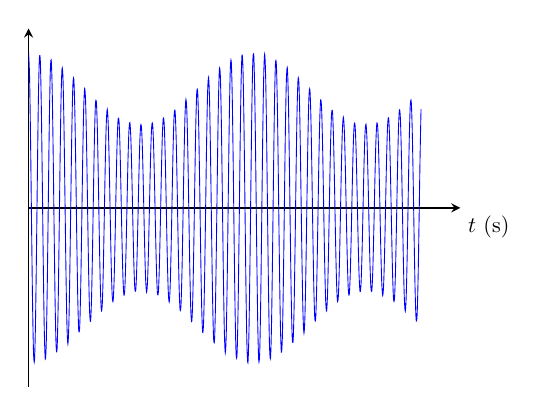
\begin{tikzpicture}[scale=0.8]
      \begin{axis}[
          ymin=-1.5, ymax=1.5,
          xmin=0, xmax=11,
          %enlargelimits,
          axis x line=center,
          axis y line=center,
          xlabel={$t$ (s)},
          xlabel style={below right},
          %label style = {at={(ticklabel cs:1.1)}}
          ticks=none,
          axis line style=thick,
        ]
        \addplot expression[samples=400,domain=0:10, mark=none, smooth] {cos(2*pi*200*x)*(1+0.3*cos(2*pi*10*x))};
      \end{axis}
    \end{tikzpicture}
    \caption{Taux de modulation $h=0.3$}
  \end{subfigure}\hfill
  \begin{subfigure}[t]{.3\linewidth}
    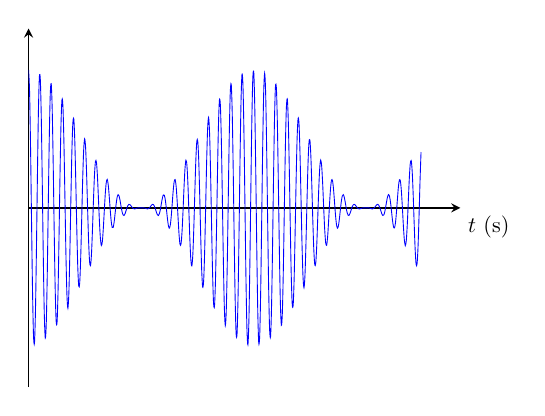
\begin{tikzpicture}[scale=0.8]
      \begin{axis}[
          ymin=-2.6, ymax=2.6,
          xmin=0, xmax=11,
          %enlargelimits=true,
          axis x line=center,
          axis y line=center,
          xlabel={$t$ (s)},
          xlabel style={below right},
          %label style = {at={(ticklabel cs:1.1)}}
          ticks=none,
          axis line style=thick,
        ]
        \addplot expression[samples=400,domain=0:10, mark=none, smooth] {cos(2*pi*200*x)*(1+1*cos(2*pi*10*x))};
      \end{axis}
    \end{tikzpicture}
    \caption{Taux de modulation $h=1$}
  \end{subfigure}\hfill
  \begin{subfigure}[t]{.3\linewidth}
    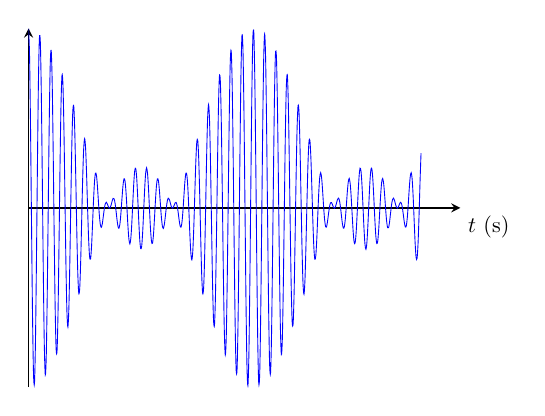
\begin{tikzpicture}[scale=0.8]
      \begin{axis}[
          ymin=-2.6, ymax=2.6,
          xmin=0, xmax=11,
          %enlargelimits=true,
          axis x line=center,
          axis y line=center,
          xlabel={$t$ (s)},
          xlabel style={below right},
          %label style = {at={(ticklabel cs:1.1)}}
          ticks=none,
          axis line style=thick,
        ]
        \addplot expression[samples=400,domain=0:10, mark=none, smooth] {cos(2*pi*200*x)*(1+1.6*cos(2*pi*10*x))};
      \end{axis}
    \end{tikzpicture}
    \caption{Taux de modulation $h=1.6$}
  \end{subfigure}\hfill
  \caption{Signaux modulés en amplitude avec différents taux de modulation.}
\end{figure}

La modulation en amplitude est la multiplication de deux signaux. La multiplication est une opération non-linéaire qui modifie leur spectre.

\subsection{Point de vue spectral}

\formule{Spectre d'un signal sinusoïdal modulé en amplitude}
[
  \begin{itemize}
    \item $s(t)$ est un signal sinusoïdal
    \item $f_p \gg f$
  \end{itemize}
]
{\schema{}{4cm}}
[
  \begin{itemize}
    \item $A_p$ l'amplitude de la porteuse (en \unit{V})
    \item $A_s$ l'amplitude du signal à transmettre (en \unit{V})
    \item $k$ le facteur multiplicatif du multiplieur (en \unit{V^{-1}})
    \item $f_p$ la fréquence de la porteuse (en \unit{Hz})
    \item $f_s$ la fréquence du signal à transmettre (en \unit{Hz})
  \end{itemize}
]
[o][o]

\formule{Spectre d'un signal quelconque modulé en amplitude}
[
  \begin{itemize}
    \item $f_p \gg f$
  \end{itemize}
]
{\schema{}{4cm}}
[
  \begin{itemize}
    \item $A_p$ l'amplitude de la porteuse (en \unit{V})
    \item $k$ le facteur multiplicatif du multiplieur (en \unit{V^{-1}})
    \item $f_p$ la fréquence de la porteuse (en \unit{Hz})
    \item $f_{max}$ la fréquence maximale présence dans le spectre du signal à transmettre (en \unit{Hz})
  \end{itemize}
]
[o][o]

\flashcard{$\cos(a)\cos(b)$}{$\frac{\cos(a+b)+\cos(a-b)}{2}$}

La \textbf{largeur de bande} est la plage de fréquence occupée par le signal modulé.

\application{Combien peut-il y avoir de stations de radio en grandes ondes (GO) ? Et dans le bande FM ?}

\section{Démodulation}
\subsection{Principe}

La démodulation est l'opération inverse de la modulation. La démodulation permet de retrouver le signal à transmettre à partir du signal modulé.

La démodulation ne peut pas être un opération linéaire car il faut modifier le spectre pour retrouver celui du signal à transmettre.

\subsection{Démodulation synchrone}

\subsubsection{Première étape : multiplication par la porteuse}

\formule{Spectre du signal après multiplication par la porteuse}
[
  \begin{itemize}
    \item $f_p \gg f_s$
    \item le signal à transmettre est sinusoïdal
  \end{itemize}
]
{\schema{}{3cm}}
[
  \begin{itemize}
    \item $A_p$ l'amplitude de la porteuse (en \unit{V})
    \item $k$ le facteur multiplicatif du multiplieur (en \unit{V^{-1}})
    \item $f_p$ la fréquence de la porteuse (en \unit{Hz})
    \item $f_s$ la fréquence du signal à transmettre (en \unit{Hz})
  \end{itemize}
]
[][o]

\colle{Dans le cas d’un signal de départ sinusoïdal, déterminer et tracer le spectre du signal modulé en amplitude puis du produit du signal modulé et de la porteuse.}

\subsubsection{Deuxième étape : filtrage passe-bas}

\formule{Spectre du signal après multiplication par la porteuse et filtrage passe bas}
[
  \begin{itemize}
    \item $f_p \gg f_s$
    \item le signal à transmettre est sinusoïdal
  \end{itemize}
]
{\schema{}{3cm}}
[
  \begin{itemize}
    \item $A_p$ l'amplitude de la porteuse (en \unit{V})
    \item $k$ le facteur multiplicatif du multiplieur (en \unit{V^{-1}})
    \item $f_p$ la fréquence de la porteuse (en unit{Hz})
    \item $f_s$ la fréquence du signal à transmettre (en unit{Hz})
  \end{itemize}
]
[][o]

\application{Quelle fréquence de coupure le filtre passe-bas peut-il avoir pour démoduler la radio en grandes ondes (GO) ?}

\subsubsection{Troisième étape : filtrage passe-haut}

\formule{Spectre du signal après démodulation}
[
  \begin{itemize}
    \item $f_p \gg f$
    \item le signal à transmettre est sinusoïdal
  \end{itemize}
]
{\schema{}{3cm}}
[
  \begin{itemize}
    \item $A_p$ l'amplitude de la porteuse (en \unit{V})
    \item $k$ le facteur multiplicatif du multiplieur (en \unit{V^{-1}})
    \item $f_p$ la fréquence de la porteuse (en unit{Hz})
    \item $f_{max}$ la fréquence maximale présence dans le spectre du signal à transmettre (en unit{Hz})
  \end{itemize}
]
[][o]

\application{Quelle fréquence de coupure le filtre passe-haut peut-il avoir pour démoduler la radio en grandes ondes (GO) ?}

\subsubsection{Schéma récapitulatif}

\schema{Démodulation synchrone}{10cm}

\colle{Pour un signal de départ sinusoïdal de fréquence $f$, représenter sur un schéma les différentes étapes de la démodulation synchrone en précisant les exigences sur les fréquences de coupure et en représentant leurs effets sur le spectre du signal.}

\colle{Pour un signal de départ audio, représenter sur un schéma les différentes étapes de la démodulation synchrone en précisant les exigences sur les fréquences de coupure et en représentant leurs effets sur le spectre du signal.}